
%%\documentclass[12pt,preprint]{aastex}

%% manuscript produces a one-column, double-spaced document:

%% \documentclass[10pt,manuscript]{aastex}

%% preprint2 produces a double-column, single-spaced document:
\documentclass[preprint2,iop,numberedappendix]{emulateapj}
%% \documentclass[preprint2,iop]{aastex}

%% \documentclass[preprint2,longabstract]{aastex}

%% \usepackage{ccaption}
%% \captionstyle{\raggedright}
\usepackage[caption=false]{subfig}
\usepackage{amsmath}
\usepackage{footnote}
\bibpunct{(}{)}{;}{a}{}{,} 
\captionsetup{belowskip=12pt,aboveskip=4pt}
\setlength{\textfloatsep}{10pt plus 1.0pt minus 2.0pt}
\newcommand{\dif}{\mathrm{d}}
%% \renewcommand*{\thefootnote}{\fnsymbol{footnote}}

\def\nar{{New~A~Rev.}}          % New Astronomy Review
\def\pasa{{PASA}}               % Publications of the Astron. Soc. of Australia

%% \bibliographystyle{mn2e}
%% \bibliographystyle{apj}

\shorttitle{Foreground signatures in EoR power spectra}
\shortauthors{Thyagarajan et~al.}

\def\ASU{\altaffilmark{1}}
\def\ASUtxt{\altaffiltext{1}{Arizona State University, Tempe, AZ 85287, USA; e-mail: t\_nithyanandan@asu.edu}}

% \def\RRI{\altaffilmark{1}}
% %% \def\RRItxt{\altaffiltext{1}{Raman Research Institute, Bangalore, India}}
% \def\RRItxt{\altaffiltext{1}{Raman Research Institute, Bangalore, India; e-mail: nithya.rri@gmail.com}}

% \def\NRAONM{\altaffilmark{2}}
% \def\NRAONMtxt{\altaffiltext{2}{National Radio Astronomy Observatory, Socorro, NM, USA}}

% \def\CAASTRO{\altaffilmark{3}}
% \def\CAASTROtxt{\altaffiltext{3}{ARC Centre of Excellence for All-sky Astrophysics (CAASTRO), Sydney, Australia}}

% \def\Curtin{\altaffilmark{4}}
% \def\Curtintxt{\altaffiltext{4}{Curtin University, Perth, Australia}}

% %% \def\Swinburne{\altaffilmark{4}}
% %% \def\Swinburnetxt{\altaffiltext{4}{Swinburne University of Technology, Melbourne, Australia}}

% \def\CfA{\altaffilmark{5}}
% \def\CfAtxt{\altaffiltext{5}{Harvard-Smithsonian Center for Astrophysics, Cambridge, USA}}

% \def\ANU{\altaffilmark{7}}
% \def\ANUtxt{\altaffiltext{7}{The Australian National University, Canberra, Australia}}

% \def\CSIRO{\altaffilmark{8}}
% \def\CSIROtxt{\altaffiltext{8}{CSIRO Astronomy and Space Science, NSW, Australia}}

% \def\Haystack{\altaffilmark{9}}
% \def\Haystacktxt{\altaffiltext{9}{MIT Haystack Observatory, Westford, USA}}

% \def\USydney{\altaffilmark{10}}
% \def\USydneytxt{\altaffiltext{10}{Sydney Institute for Astronomy, School of Physics, The University of Sydney, Sydney, Australia}}

% \def\MIT{\altaffilmark{11}}
% \def\MITtxt{\altaffiltext{11}{MIT Kavli Institute for Astrophysics and Space Research, Cambridge, USA}}

% \def\UW{\altaffilmark{12}}
% \def\UWtxt{\altaffiltext{12}{University of Washington, Seattle, USA}}

% \def\Victoria{\altaffilmark{13}}
% \def\Victoriatxt{\altaffiltext{13}{Victoria University of Wellington, Wellington, New Zealand}}

% \def\UWisc{\altaffilmark{14}}
% \def\UWisctxt{\altaffiltext{14}{University of Wisconsin--Milwaukee, Milwaukee, USA}}

% \def\UMelbourne{\altaffilmark{15}}
% \def\UMelbournetxt{\altaffiltext{15}{The University of Melbourne, Melbourne, Australia}}

% \def\Tata{\altaffilmark{16}}
% \def\Tatatxt{\altaffiltext{16}{Tata Institute of Fundamental Research, Pune, India}}

% \def\NRAOGBT{\altaffilmark{17}}
% \def\NRAOGBTtxt{\altaffiltext{17}{National Radio Astronomy Observatory, Charlottesville, USA}}

% \def\UTasmania{\altaffilmark{18}}
% \def\UTasmaniatxt{\altaffiltext{18}{University of Tasmania, Hobart, Australia}}

% \def\UWA{\altaffilmark{19}}
% \def\UWAtxt{\altaffiltext{19}{University of Western Australia, Perth, Australia}}

% %% \def\ICRAR{\altaffilmark{9}}
% %% \def\ICRARtxt{\altaffiltext{9}{International Centre for Radio Astronomy Research, Curtin University, Perth, Australia }}

% %\def\VUW{\altaffilmark{13}}
% %\def\VUWtxt{\altaffiltext{13}{Victoria University of Wellington, New Zealand}}

%% \definenote[thanks][conversion=set 2]

\begin{document}

%% \title{Detecting Epoch of Reionization in redshifted 21~cm: contamination in EoR window}
%% \title{Limits on the detection of the Epoch of Reionization from MWA observations of the redshifted 21~cm line}
\title{Signatures of Foreground Sky in Power Spectra of Redshifted Neutral Hydrogen from the Epoch of Reionization}

%% Use \author, \affil, and the \and command to format
%% author and affiliation information.
%% Note that \email has replaced the old \authoremail command
%% from AASTeX v4.0. You can use \email to mark an email address
%% anywhere in the paper, not just in the front matter.
%% As in the title, use \\ to force line breaks.

%% \author{NITHYANANDAN~THYAGARAJAN\altaffilmark{1}, 
%%   N.~UDAYA~SHANKAR\altaffilmark{1}, 
%%   \and RAVI~SUBRAHMANYAN\altaffilmark{1}}


%% Author list
\author{
%% Lead authors
Nithyanandan~Thyagarajan\ASU,
Daniel~C.~Jacobs\ASU,
Judd~D.~Bowman\ASU
}

%Institutional footnotes (typeset, then rearrange here to be in order)
\ASUtxt
% \RRItxt
% \NRAONMtxt
% \CAASTROtxt
% \Curtintxt
% %% \Swinburnetxt
% \CfAtxt
% \ANUtxt
% \CSIROtxt
% \Haystacktxt
% \USydneytxt
% \MITtxt
% \UWtxt
% \Victoriatxt
% \UWisctxt
% \Tatatxt
% \NRAOGBTtxt
% \UMelbournetxt
% \UTasmaniatxt
% %% \UWAtxt
% %% \ICRARtxt
% %\VUWtxt

%% \email{t\_nithyanandan@rri.res.in}

%% \clearpage

\begin{abstract}

We characterize signatures of foreground radio emission and instrument configuration on the observed power spectra of redshifted H{\sc i} 21~cm line emission from the epoch of reionization (EoR) using a baseline (antenna pair) based ``delay spectrum'' analysis technique. We use the 128-tile Murchison Widefield Array (MWA) instrument configuration for our studies. % Our analysis is centered around 185~MHz with 30.72~MHz bandwidth at 80~kHz frequency resolution. 
We simulate the delay spectrum response of interferometers, for the first time, to an all-sky foreground model consisting of diffuse (on scales $\gtrsim\,$0\fdg 85) and compact Galactic and extragalactic emission. By tying model parameters to those of a subset of first season of observing with the MWA, the ratio of our predictions to observations, subject to expected errors, are consistent with unity at $\gtrsim$~90\% confidence level. A wedge-shaped region of foreground contamination and a spillover from this contamination into relatively foreground--free regions ({\it EoR window}) in the delay spectrum due to spectral properties of foreground emission and the instrument is confirmed. Due to shortening of antenna spacings caused by projection effects, diffuse emission produces edge-heavy features in the wedge even on large antenna spacings, hitherto not predicted. Features in the inner regions of the wedge are predominantly due to compact foreground objects. This results in a ``pitchfork'' shaped delay spectrum. We also provide a practical diagnostic tool for data analysis that helps in identifying interferometers with high foreground contamination.

\end{abstract}
 
\keywords{large-scale structure of Universe --- methods: statistical --- radio continuum: galaxies --- radio lines: general --- reionization --- techniques: interferometric}

\section{Introduction}\label{intro}

After the CMB epoch, the period in the history of the universe often referred to as the {\it dark ages}, followed the epoch of reionization (EoR). This was a period of non-linear growth of density perturbations and astrophysical evolution. Studying the epoch of reionization holds the key to understanding this evolution. Recently, observing the redshifted 21~cm spin transition of neutral hydrogen has emerged as a very promising experiment to fill the gaps in our understanding of the universe's history.  

Sensitive instruments such as the Square Kilometer Array (SKA) are required for direct observation and tomography of redshifted H{\sc i}. Numerous precursors to the SKA such as the Murchison Widefield Array \citep[MWA;][]{lon09,tin13}, the Low Frequency Array \citep[LOFAR;][]{van13}, and the Precision Array for Probing the Epoch of Reionization \citep[PAPER;][]{par10} have become operational with enough sensitivity for a statistical detection of the EoR H{\sc i} power spectrum. 

One of the key challenges in the statistical detection of power spectrum of the redshifted H{\sc i} signal arises from the contamination by Galactic and extragalactic foregrounds \citep[see, e.g.,][]{dim02,zal04,fur06}. \citet{mor04} show that the inherent isotropy and symmetry of the EoR signal in frequency and spatial wavenumber ($k$) space make it distinguishable from sources of contamination which lack such symmetry. Foreground removal techniques rely on the spectral smoothness of foreground emission \citep{mor06,bow09,liu11,par12,dil13}.

Precise understanding of these foreground signatures is necessary in order to remove foreground systematics from the measured power spectrum. Considerable effort has been made in mapping the residual foreground signatures in observed power spectrum \citep{thy13,pob13,mor12,tro12,dat10,bow09} after foreground subtraction. 

In this paper, in one of the most detailed characterizations to date, using an interferometer (antenna pair) based delay spectrum technique, we demonstrate the signatures of unsubtracted diffuse and compact foreground models in delay spectrum, a quantity closely related to the sought power spectrum. The simplicity of this technique and usage of basic interferometric visibility data fourier transformed along frequency (delay spectrum) on individual interferometers offer very effective diagnostics for scheduling observations and data analysis, and an insightful view onto foreground signatures in the EoR H{\sc i} power spectrum. We explore the diversity in these signatures as a function of observation and instrument parameters and confirm our findings with data obtained from the MWA. This simple technique allows us to predict foreground signatures, hitherto not predicted. 

We have organized this paper as follows. \S\ref{sec:delay-spectrum} defines the delay spectrum and its relation to the power spectrum. \S\ref{sec:instrument} and \S\ref{sec:obsparms} describe the MWA instrumental parameters and observation parameters used in this study respectively. Analysis of data obtained with the MWA is described in \S\ref{sec:data-analysis}. In \S\ref{sec:modeling}, we describe the building blocks of our delay spectrum modeling including the models used for the antenna power pattern and foreground. Here, we also establish that the results of modeling and data analysis agree with each other. In \S\ref{sec:delay-spectrum-analysis}, we present a detailed analysis of the signatures of foregrounds on the modeled delay spectrum and its dependence on instrumental and observation parameters. In \S\ref{sec:fg-grading}, we use our understanding to grade interferometers based on the amount of foreground contamination estimated by the delay spectrum technique. In \S\ref{sec:summary}, we present our summary and conclusions.

\section{Delay Spectrum}\label{sec:delay-spectrum}

Interferometer array data known as {\it visibilities}, $V_f(\overline{\mathbf{u}},f)$, represent correlations between time--series of electric fields measured by different antenna pairs with separation vectors $\overline{\mathbf{x}}$ and then Fourier transformed along time axis to obtain a spectrum along frequency ($f$) axis. Here, $\overline{\mathbf{u}}\equiv \overline{\mathbf{x}}f/c \equiv \overline{\mathbf{x}}/\lambda$, $c$ is the speed of light and $\lambda$ is the wavelength. $\overline{\mathbf{u}}$ is related to transverse spatial frequency modes ($\overline{\mathbf{k}}_\perp$) of brightness distribution of the sky as $\overline{\mathbf{k}}_\perp \equiv 2\pi\overline{\mathbf{u}}/D(z)$, where $D(z)$ is the transverse comoving distance at a redshift $z$. If $I(\overline{\mathbf{l}},f)$ is the emission at different frequencies on the sky as a function of direction unit vector ($\overline{\mathbf{l}}$) specified as direction cosines, $V_f(\overline{\mathbf{u}},f)$ represents the Fourier decomposition of $I(\overline{\mathbf{l}},f)$ attenuated by the antenna's angular power pattern $A(\overline{\mathbf{l}},f)$, into transverse spatial frequency modes. Taking into account the instrumental bandpass weights $W_f(f)$, this relation can be written as:
\begin{align}\label{eqn:obsvis}
  V_f(\overline{\mathbf{u}},f) &= \int A(\overline{\mathbf{l}},f)\,I(\overline{\mathbf{l}},f)\,W_f(f)\,e^{-i2\pi \overline{\mathbf{u}}\cdot\overline{\mathbf{l}}}\,\dif^2 \overline{\mathbf{l}}.
\end{align}

We define the {\it delay spectrum} $V_\eta(\overline{\mathbf{u}},\eta)$ to be the inverse Fourier transform of $V_f(\overline{\mathbf{u}},f)$ along the frequency coordinate:
\begin{align}\label{eqn:delay-transform}
  V_\eta(\overline{\mathbf{u}},\eta) &= \int V_f(\overline{\mathbf{u}},f)\,W'_f(f)\,e^{i2\pi\eta f}\,\dif f,
\end{align}
where, $W'_f(f)$ is a frequency window weighting function which can be chosen to control the quality of the delay spectrum \citep{thy13,ved12}. $\eta$ represents the signal delay between the antenna pairs in an interferometer given by:
\begin{equation}\label{eqn:delay}
  \eta = \frac{\overline{\mathbf{x}}\cdot\overline{\mathbf{l}}}{c} = \frac{\overline{\mathbf{u}}\cdot\overline{\mathbf{l}}}{f}.
\end{equation}
The terms delay and lag are used interchangeably in this paper.

Since we are studying a redshifted H{\sc i} spectral line, $f$ is a measure of cosmological distance along the line of sight. Consequently, $\eta$ is a measure of line of sight spatial frequency mode, $k_\parallel$. Thus, $|V_\eta(\overline{\mathbf{u}},\eta)|^2$ is directly related to the spatial power spectrum of redshifted H{\sc i} distribution, $|V(\overline{\mathbf{k}}_\perp,k_\parallel)|^2$. However, foreground objects emit in radio frequencies and contaminate the signals from the redshifted H{\sc i}. Due to their spatial and spectral properties, $V_\eta(\overline{\mathbf{u}},\eta)$ also contains contamination from foreground radio sources \citep{thy13,tro12,mor12,bow09}. These contaminations have to be characterized precisely in order to reduce their impact on redshifted H{\sc i} power spectrum detection sensitivity. 

In summary, $V_\eta(\overline{\mathbf{u}},\eta)$, is closely related to visibilities, $V_f(\overline{\mathbf{u}},f)$, the basic data blocks measured by an interferometer, as seen from equation~\ref{eqn:delay-transform}. It captures all the effects of EoR H{\sc i} signal corruption caused by foregrounds and the instrument. At the same time, it is very closely related to the sought power $|V(\overline{\mathbf{k}}_\perp,k_\parallel)|^2$ in $k$--modes. For our analysis, we use an equivalent quantity, $V_\eta(\overline{\mathbf{x}},\eta) \equiv V_\eta(\lambda\overline{\mathbf{u}},\eta)$. For purposes of illustration, we often use a simplified quantity $|V_\eta(|\overline{\mathbf{x}}|,\eta)|$.

We now describe in detail an important ingredient, the MWA instrument.

\section{Instrument Parameters}\label{sec:instrument}

We use the 128-tile layout of the MWA \citep{bea12} and choose a center frequency of 185~MHz with a bandwidth of 30.72~MHz divided into 384 frequency channels each of width 80~kHz. The choice of center frequency translates to $z\approx 6.68$ for the 21~cm spin flip transition of H{\sc i}. The bandwidth was chosen to be close to the maximum instantaneous value of the MWA in order to maximize the resolution in delay coordinates and obtain detailed characteristics of delay spectra from foregrounds. We restrict our analysis to the innermost antenna spacings with $|\overline{\mathbf{x}}| \leq x_\textrm{max} = 200$~m, or $|\overline{\mathbf{u}}| \leq u_\textrm{max} = 123$ at a frequency of 185~MHz. These interferometers are responsive to transverse spatial structures on scales $\gtrsim 1/u_\textrm{max} \approx 28$\arcmin. Hereafter, we use the terms tile and antenna interchangeably to refer to the MWA tile. 

The bandpass weights in the frequency window of the MWA are obtained through a 8-tap Polyphase Filter Bank (PFB) using a Kaiser window with the $\beta$ parameter set to 5. The bandpass weights consist of coarse frequency channels of width 1.28~MHz each of which contains 16 finer frequency channels of width 80~kHz. Our analysis, therefore, contains 24 coarse channels. As the data are subsequently bandpass calibrated, the bandpass weights are normalized to unity. But the edges of the coarse channels are noisy and aliased from adjacent coarse channels. Thus, we remove one fine channel from each side of the coarse channel edges from our data. This constitutes $W_f(f)$ in equation~\ref{eqn:obsvis}. The bandpass properties used in this paper are illustrated in figure~\ref{fig:bandpass}. 

\begin{figure}[htb]
\centering
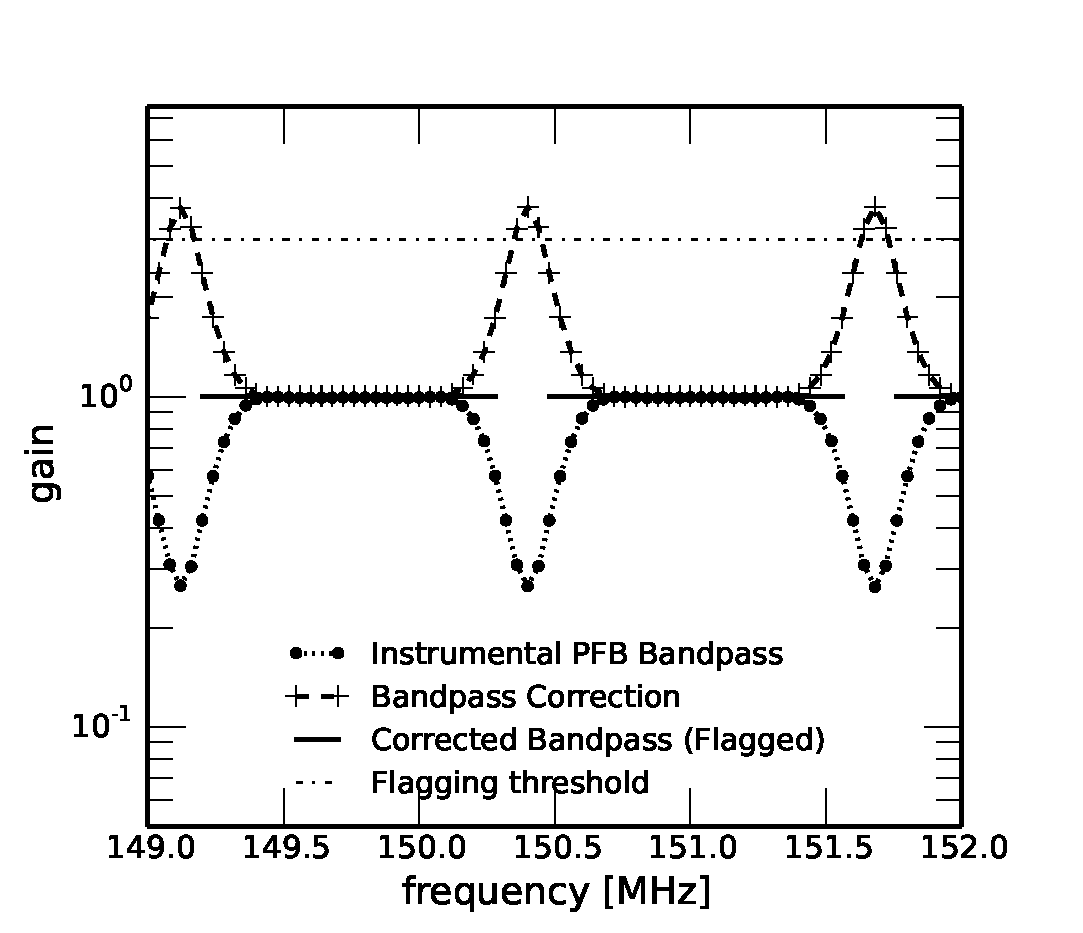
\includegraphics[width=\linewidth]{figures/v1_0/bandpass_properties}
\caption{Bandpass properties used in modeling and analysis of delay spectrum of MWA visibilities. The filled circles joined by dotted lines show the 8-tap PFB bandpass shapes obtained using a Kaiser window with parameter $\beta=5$. The {\it plus} symbols joined by dashed lines are the bandpass correction factors. The solid line shows the flagged (gaps) and gain--corrected bandpass shape, $W_f(f)$. These shapes are repeated every 1.28~MHz for the entire bandwidth of 30.72~MHz centered around 185~MHz. \label{fig:bandpass}}
\end{figure}

Thermal noise in simulated visibilities is estimated assuming a system temperature of $T_\textrm{sys}=90$~K per polarization for all frequency channels for all interferometers throughout the course of observation. We take into account the increase in thermal uncertainty in frequency channels that results due to aforementioned bandpass correction. 

\section{Observation Parameters}\label{sec:obsparms}

One of the primary targets for EoR observing with the MWA is a patch of sky centered around RA = 00h 00m 00.00s, Dec = -30\arcdeg$\,$00\arcmin$\,$00\farcs 0. This is one of the regions of low foreground emission within 27\arcdeg$\,$ from the zenith. The MWA tracks a patch of sky through antenna beams formed and steered electronically by controlling delay settings of an array of dipoles in a MWA tile. These beamformer delay settings can be changed only in discrete steps. Accordingly, observations were made in a ``drift and shift'' (D-S) mode. Figure~\ref{fig:pointings} shows the direction of pointing of MWA tiles during the course of the observation. The sky is allowed to drift for a certain period of time (usually $\sim 30$~mins) before the discrete shifts in the beamformer delay settings position the beam to be centered again on the same patch of sky. This process is repeated throughout the course of the observation $\approx 4.86$~hours. The LST of two snapshots we chose for our study are shown as vertical lines at -1.92~hours (wrapped by 360\arcdeg from 22.08~hours) and 0.09~hours which are hereafter denoted as {\it off--zenith} and {\it zenith} pointings respectively. These pointings (phased array power patterns) are centered at RA = 4\fdg 387, Dec = -29\fdg 86 and RA = -28\fdg 8, Dec = -26\fdg 701, whereas the visibilities themselves are phased to zenith corresponding to RA = -28\fdg 8, Dec = -26\fdg 701, and RA = 1\fdg 35, Dec = -26\fdg 701 respectively. 

\begin{figure}[htb]
\centering
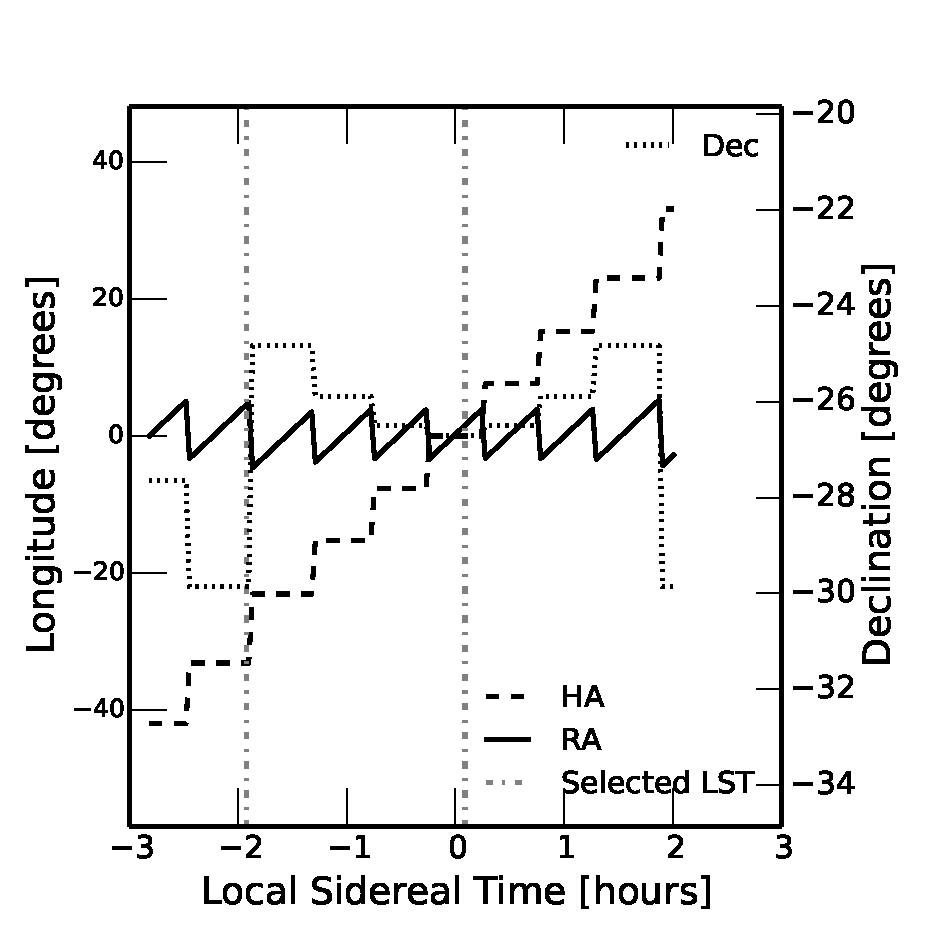
\includegraphics[width=\linewidth]{figures/v1_0/custom_pointings.eps}
\caption{MWA tile beam pointing directions during the course of the observation. The x-axis refers to the Local Sidereal Time (LST) in hours. The axis on the left refers to longitudes, namely, Right Ascension (RA) and Hour Angle (HA) in degrees. Negative values of RA, HA, and LST are to be interpreted as having been wrapped around by 360\arcdeg or 24 hours. The axis on the right refers to the declination of the pointing direction. The RA, HA, and declination are plotted with solid, dashed and dotted line styles respectively. A ``drift and shift'' scheme is used. The sky is allowed to drift for $\sim 30$~mins before the beamformer delay settings change in a discrete step to center the beam around RA = 00h 00m 00.00s, Dec = -30\arcdeg$\,$00\arcmin$\,$00\farcs 0. Dot--dashed vertical lines show the LST of off-zenith and zenith pointings used in our study. \label{fig:pointings}}
\end{figure}

Throughout this paper, $\overline{\mathbf{u}}$ and $\overline{\mathbf{x}}$ are assumed to be on a coordinate system aligned with the local east and north (along local meridian) directions at the MWA site. For the conventions of Fourier transform and its inverse we use in this paper, in accordance with equation~\ref{eqn:delay}, signals from the sky towards east and north are recorded with positive delays on eastward and northward oriented antenna spacings respectively. For instance, at the beginning of the observation, the Galactic center is in the westward sky just about to set. Signals from this direction are recorded with a negative delay on interferometers whose antenna spacings are oriented towards the east. Similarly, signals from directions eastward of the local meridian arrive with positive delays on eastward oriented antenna spacings. 

For geometrical intuition, we restrict the orientation ($\theta_b$, measured anti-clockwise from East) of all antenna spacings to lie in the range $-67\fdg 5 \leq \theta_b < 112\fdg 5$. Interferometers with antenna spacings oriented in the other half-plane measure conjugate visibilities with delays of equal magnitude but of opposite sign and hence are ignored in our analysis.

\section{Data Analysis}\label{sec:data-analysis}

\subsection{Imaging and deconvolution}\label{sec:FHD}

{\bf Describe the FHD data analysis up to the point of getting calibrated visibilities here.}

\subsection{Deconvolution along Delay Axis}\label{sec:CLEAN}

We obtain the delay spectrum of these calibrated visibilities using equation~\ref{eqn:delay-transform} while choosing $W'_f(f)$ to be a {\it Blackman--Harris} window function. Due to periodic gaps in frequency bandpass occurring in intervals of 1.28~MHz (see figure~\ref{fig:bandpass}), the delay spectrum is expected to contain harmonics of actual foreground emission repeated at intervals of 0.78~$\mu$s. Hence, we have employed deconvolution by {\it CLEAN} algorithm \citep{tay99} along the delay axis \citep{par09,par12} to rid the delay spectra of such artifacts. The convolving kernel for the algorithm is given by the inverse Fourier transform of the instrumental bandpass shape. 

\subsection{Delay Spectrum after Delay Deconvolution}\label{sec:data-delay-spectrum}

We show results of delay spectrum from MWA data after deconvolution along delay axis in figure~\ref{fig:fhd_data}. Boundaries of the {\it foreground wedge} are also shown. The {\it off--zenith} pointing has emission notably higher than in the {\it zenith} pointing inside the wedge boundaries. This is shown later to be due to response of the interferometer array to the bright Galactic center and Galactic plane in the westward sky. Consequently, the contamination into the {\it EoR window} is also higher. Emission in {\it zenith} pointing is more centrally concentrated due to phasing of power pattern to the zenith, whereas the {\it off--zenith} pointing has a power pattern phased eastward of zenith and is also responsive to emission from angles far away from zenith. 

\begin{figure}[htb]
\centering
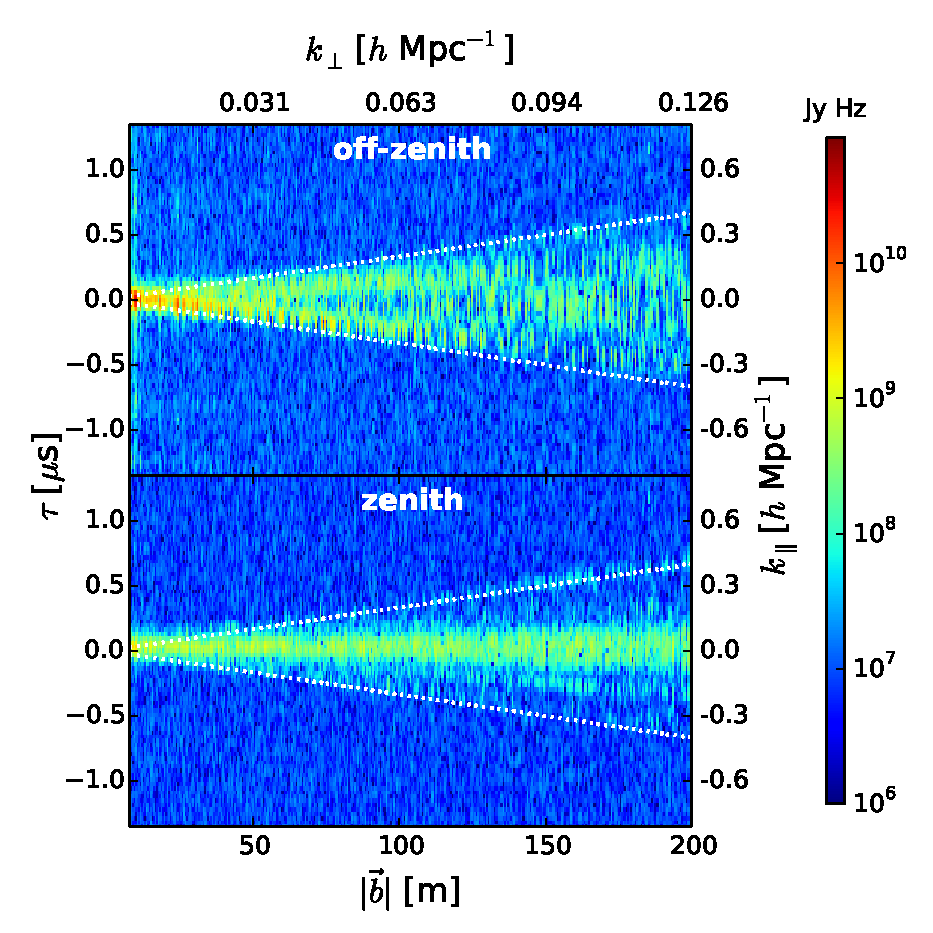
\includegraphics[width=\linewidth]{figures/v1_0/multi_baseline_fhd_delay_spectrum_snapshots.eps}
\caption{Delay spectrum amplitude, $|V_\eta(|\overline{\mathbf{x}}|,\eta)|$ (in units of Jy~Hz), obtained with MWA data for {\it off--zenith} (top) and {\it zenith} (bottom) pointings. White lines mark the boundaries of {\it foreground wedge} determined by the horizon limit and antenna spacing. The features in the wedge appear to be brighter and the spillover contamination appears to be higher in the {\it off--zenith} pointing relative to the {\it zenith} pointing due to the presence of brighter foregrounds such as the Galactic center and the Galactic plane. The logarithmic color scale (shown at the right) is common to both panels.\label{fig:fhd_data}}
\end{figure}

Despite delay deconvolution, we still see leakage beyond the cleaned regions indicating the inability of the deconvolution algorithm to fit the data perfectly. This is predominant at short baselines. This is because the maximum delay envelope (boundary of the wedge) consists of mixed emission from large portions of the sky into a narrow range of delays and the deconvolution algorithm does not have sufficient support in delay space to fit the delay spectrum. However, we note that the purpose of deconvolution is to rid the delay spectra of instrumental artifacts to the best extent possible in order to see the underlying signatures of foreground emission. It is not our intention in this paper to use the deconvolution as a foreground removal tool. Hence, our discussion and conclusions still hold despite imperfections in deconvolution.

\section{Delay Spectrum Modeling}\label{sec:modeling}

We describe power pattern and foreground models we have used in modeling the measured delay spectra. 

\subsection{Power pattern}\label{sec:power_pattern}

The power pattern of a MWA tile, $A(\overline{\mathbf{l}},f)$ in equation~\ref{eqn:obsvis}, over the entire hemisphere is analytically modeled based on a 4$\times$4 phased array of isotropic radiators at a height of 0.3~m above an infinite ground plane. We also assume that the delay corrections during the phased addition of dipole voltages in the beamformer suffer from random fluctuations of rms 0.05~ns. The models of power pattern used in data analysis take into account effects of mutual coupling of dipoles in the tile besides finite ground plane effects. Our models were found to be in good agreement with those used in the data analysis. 

\begin{figure}[htb]
\centering
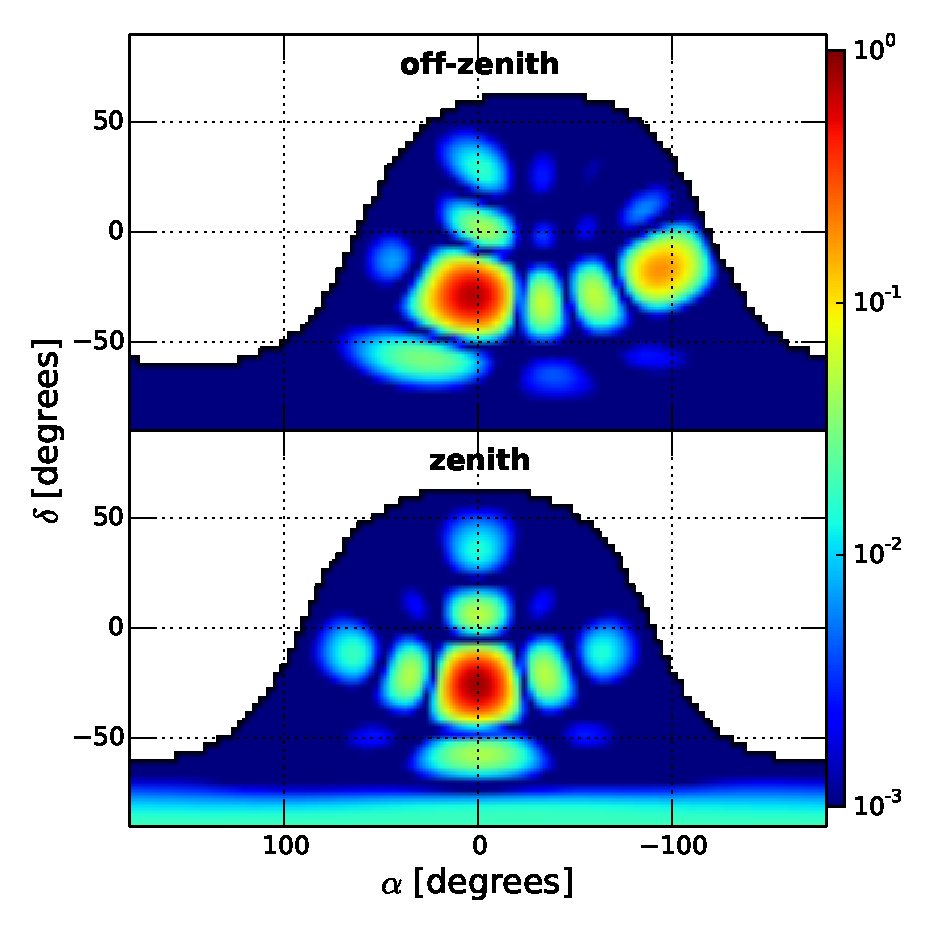
\includegraphics[width=\linewidth]{figures/v1_0/delta_array_powerpattern_0.3m_ground_custom.eps}
\caption{Models of MWA tile power pattern in Right Ascension ($\alpha$) and Declination ($\delta$) coordinates for the off--zenith (top) and zenith pointings (bottom) at 185~MHz. An MWA tile is modeled as a 4$\times$4 array of isotropic radiators placed 0.3~m above the ground plane. Random fluctutations of rms 0.05~ns have been added to delay corrections during the phased addition of voltages from these isotropic radiators. The logarithmic color scale (shown at the right) is common to both panels. \label{fig:power_pattern}}
\end{figure}

\subsection{Foreground Model}\label{sec:foreground}

An instrument such as the MWA has a very wide field of view ($\gtrsim 20$\arcdeg at 185~MHz) for imaging purposes. In the context of EoR H{\sc i} power spectrum, it has been known that unsubtracted forground sources anywhere in the visible hemisphere up to the horizon directly contaminate the spatial frequency modes in the power spectrum. In addition, this contamination also spills over into the relatively cleaner regions, called {\it EoR window}, due to spectral properties of the instrument and the foregrounds \citep{thy13,pob13,ved12,par12}. Thus, it is important to consider an all-sky model for foreground objects in evaluating the features seen in the power spectrum instead of restricting to the primary field of view. 

\citet{bea13} estimated the sensitivity of the MWA to EoR H{\sc i} power spectrum detection taking into account theremal noise effects in the {\it Eor window}. \citet{thy13} estimated the sensitivity taking into account the spillover from foreground contamination from unsubtracted extragalactic point sources in the {\t EoR window} besides thermal noise. In this paper, we include the diffuse Galactic emission for enhancing our understanding of foreground signatures in the power spectrum. We use an all-sky foreground emission model that consists of diffuse and bright compact components. 

\subsubsection{Diffuse Foreground Model}\label{sec:DSM}

For the diffuse component, we use an all-sky radio foreground model \citep{deo08} to estimate the emission at 185~MHz. Since this map is predominantly based on the 408~MHz all-sky map of \citet{has82} which has an angular resolution of 0\fdg 85, we smoothed the 185~MHz diffuse emission map to the same resolution. However, to avoid any artifacts from sampling this map, we sample it at $\approx 27$\arcmin~intervals. Using the same source model, we also obtain the diffuse emission maps at 170~MHz and 200~MHz to estimate the spectral index map of the diffuse emission model. 

A low resolution version of the diffuse foreground model used is show in figure~\ref{fig:DSM}. Contours of the MWA tile power pattern shown in figure~\ref{fig:power_pattern} are also overlaid. Of notable significance in the {\it off--zenith} pointing is the presence of a portion of the Galactic plane and the bright Galactic center in the visible hemisphere in the westward sky and the MWA tile's power receptivity is significantly high ($\gtrsim 0.125$) in that direction. In the {\it zenith} pointing, the Galactic plane has almost set and the contour level of power pattern in that direction is at least 16 times lesser. 

\begin{figure}[htb]
\centering
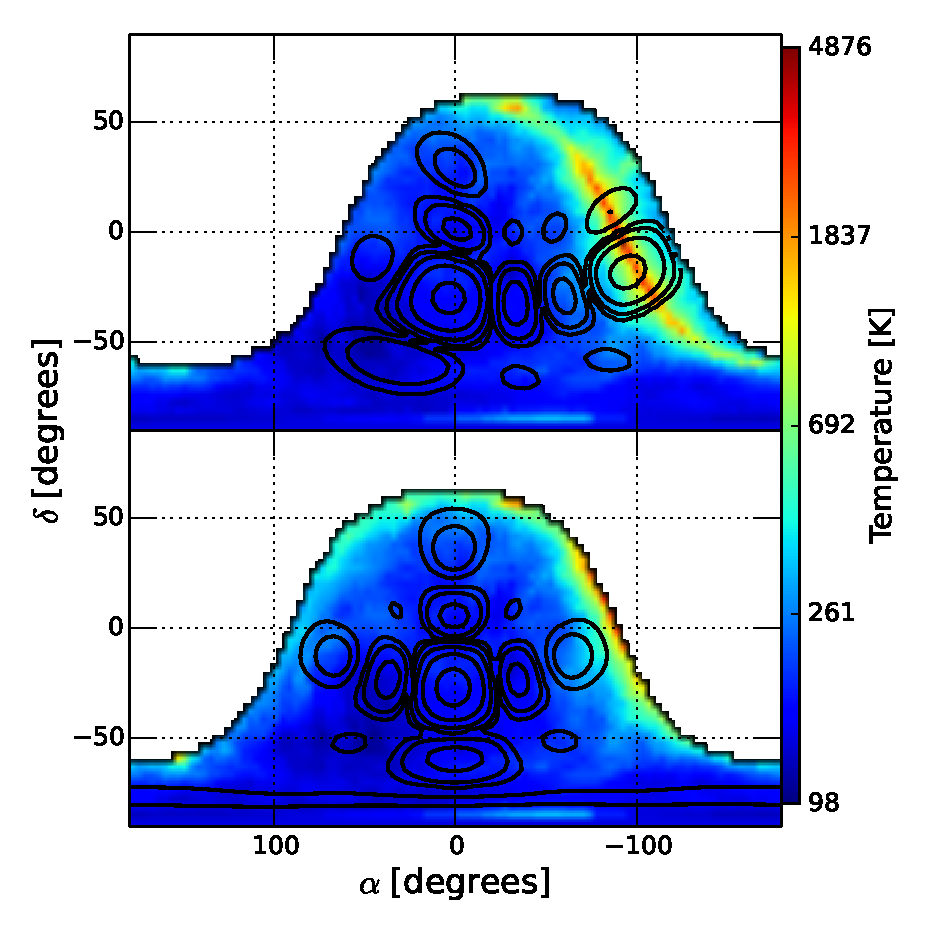
\includegraphics[width=\linewidth]{figures/v1_0/dsm.eps}
\caption{Sky brightness temperature (in K) of the diffuse foreground model at 185~MHz in Right Ascension ($\alpha$) and Declination ($\delta$) coordinates visible during {\it off--zenith} (top) and {\it zenith} (bottom) pointings. The color scale on the right is logarithmic and is common to both panels. Contours of power pattern shown in figure~\ref{fig:power_pattern} are overlaid. The contour levels shown are 0.001953125, 0.0078125, 0.03125, 0.125, and 0.5. The Galactic center and a portion of the Galactic plane are prominently visible during the {\it off--zenith} pointing and the MWA tile power receptivity is significant ($\gtrsim 0.125$) in that direction. In contrast, emission from the Galactic plane in {\it zenith} pointing is significantly lesser. \label{fig:DSM}}
\end{figure}

\subsubsection{Compact Foreground Model}\label{sec:CSM}

We use a combination of NRAO VLA Sky Survey \citep[NVSS;][]{con98} at 1.4~GHz and Sydney University Molonglo Sky Survey \citep[SUMSS;][]{boc99,mau03} at 843~MHz due to their similar flux sensitivity and angular resolution, and complimentary survey footprints covering the entire sky. The SUMSS catalog covers the sky with declination $\delta < -30$\arcdeg with a limiting peak brightness of 6--10~mJy/beam and an angular resolution of $\sim 45$\arcsec. The NVSS covers the sky with $\delta > -40$\arcdeg with a similar angular resolution and a limiting flux density of $\approx 2.5$~mJy for discrete sources. 

From the SUMSS catalog, we select compact sources whose deconvolved major axes are equal to 0. From the NVSS catalog, we excluded objects that overlap with those in the SUMSS survey footprint. Compact sources from NVSS were selected if the convolved major axes were not greater than $\approx 47$\arcsec, which is almost equal to the angular resolution of the survey. Using a mean spectral index of $\langle\alpha_\textrm{sp}\rangle=-0.83$ (flux density, $S(f)\propto f^{\alpha_\textrm{sp}}$) obtained by \citet{mau03} for both NVSS and SUMSS catalog objcts, we calculate the corresponding flux densities at 185~MHz, $S_{185}$. From this subset, we choose compact objects with $S_{185}\geq 10$~Jy. The selection of such bright compact objects is not affected by minor differences in sensitivity of the two surveys. We verified that our selection criteria ensure a similar areal density of sources in the two surveys. 

Based on these criteria, we selected 133 sources from the SUMSS catalog and 336 sources from the NVSS catalog. Together with the diffuse foreground model, we obtain an all-sky foreground model consisting of both compact and diffuse emission.

\begin{figure}[htb]
\centering
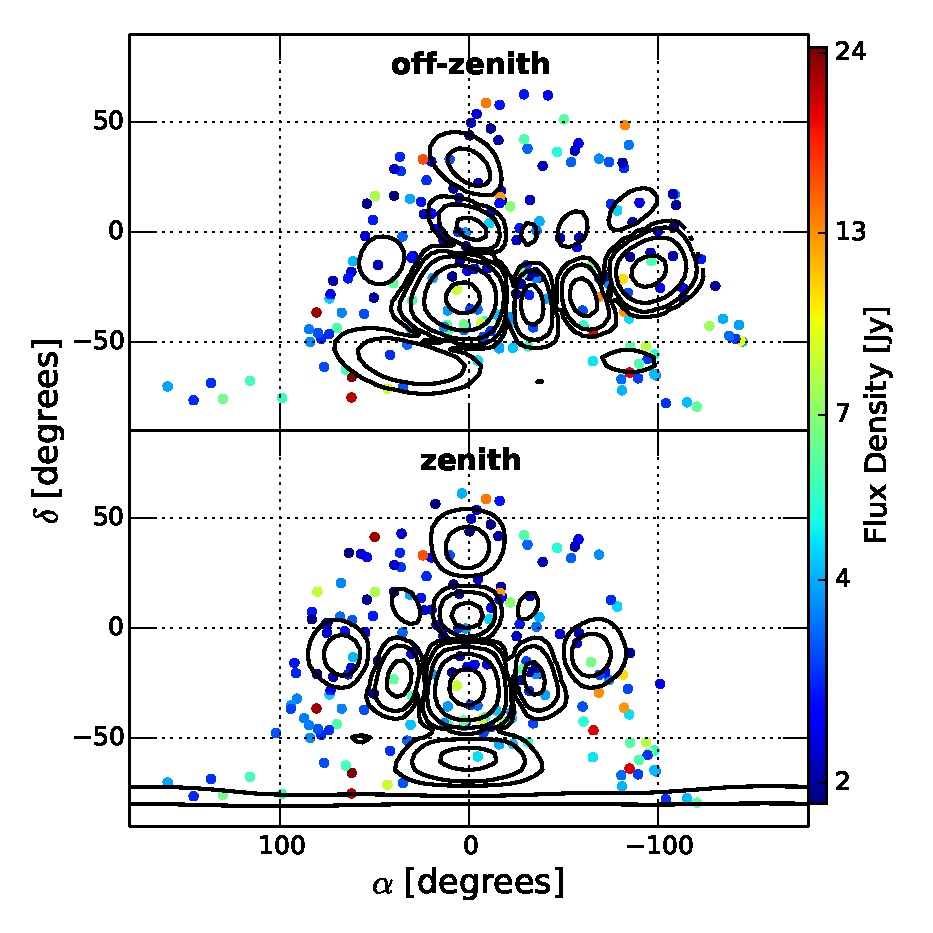
\includegraphics[width=\linewidth]{figures/v1_0/csm.eps}
\caption{Flux densities (in Jy) of bright compact sources at 185~MHz in Right Ascension ($\alpha$) and Declination ($\delta$) coordinates visible during {\it off--zenith} (top) and {\it zenith} (bottom) pointings. The color scale on the right is logarithmic and is common to both panels and corresponds to the color--coded filled circles. Contours of power pattern shown in figure~\ref{fig:power_pattern} are overlaid. The contour levels shown are 0.001953125, 0.0078125, 0.03125, 0.125, and 0.5. The locations of bright compact sources appear to be random.\label{fig:CSM}}
\end{figure}

\subsection{Comparison with Data}\label{sec:data-vs-model}

With the aforementioned all-sky foreground model, and instrumental and observational parameters, we simulate visibilities using equation~\ref{eqn:obsvis}. Figure~\ref{fig:sim_data} shows the amplitude of delay spectrum from {\it off--zenith} and {\it zenith} pointings. Notice the qualitative agreement of amplitude and structure with those obtained from data shown in figure~\ref{fig:fhd_data}. The Galactic center and the Galactic plane visible in the {\it off--zenith} pointing make it appear brighter in the {\it foreground wedge}. 

\begin{figure}[htb]
\centering
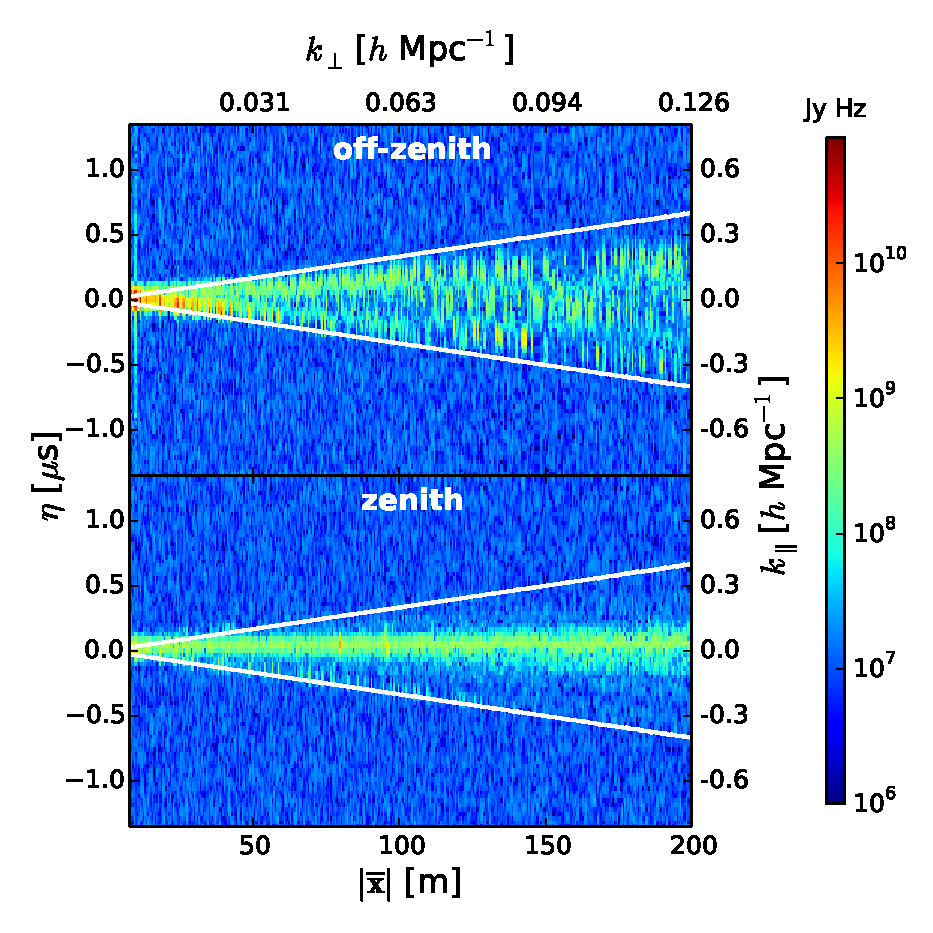
\includegraphics[width=\linewidth]{figures/v1_0/multi_baseline_sim_delay_spectrum_snapshots.eps}
\caption{Delay spectrum amplitude, $|V_\eta(|\overline{\mathbf{x}}|,\eta)|$ (in units of Jy~Hz), obtained with simulations for {\it off--zenith} (top) and {\it zenith} (bottom) pointings. White lines mark the boundaries of {\it foreground wedge} determined by the horizon limit and antenna spacing. The features resemble those obtained with MWA data shown in figure~\ref{fig:fhd_data}. The Galactic center and Galactic plane prominently visible in the {\it off--zenith} pointing makes the emission in the {\it foreground wedge} brighter relative to that in the {\it zenith} pointing. The axes and color scale are identical to those in figure~\ref{fig:fhd_data}. \label{fig:sim_data}}
\end{figure}

In order to make a quantitiative comparison of delay spectra obtained with the MWA data and our simulations, we consider the following uncertainties. Our foreground models are derived from other higher frequency catalogs and sky maps. The inherent spread in spectral index increases the uncertainty while predicting fluxes at the observing frequency. Using simple error propagation, the fractional error in the delay spectrum caused by the spread in spectral index is $\sim \ln(f_\textrm{orig}/f)\,\Delta\alpha_\textrm{sp}$, where, $f_\textrm{orig}$ is the original frequency at which the catalog or map was created, $f=185$~MHz is the observing frequency, and $\Delta\alpha_\textrm{sp}$ is the spread (HWHM) in spectral index. From \citet{mau03}, we assume $\Delta\alpha_\textrm{sp} \approx 0.35$ for compact sources from NVSS and SUMSS catalogs. We assume the same holds true for our diffuse sky model as well, which is predominantly derived from 408~MHz map of \citet{has82}. Besides, delay spectra from simulations and data each have uncertainties arising from thermal noise with rms, $\Delta V^\textrm{N}_\eta(|\overline{\mathbf{x}}|,\eta) \sim 1.4\times 10^7$~Jy~Hz, where the superscript N stands for thermal noise. We estimate the ratio of delay spectra from data and simulations as, $\rho = |V^\textrm{D}_\eta(|\overline{\mathbf{x}}|,\eta)|/|V^\textrm{S}_\eta(|\overline{\mathbf{x}}|,\eta)|$, where superscripts D and S denote data and simulation respectively. Using the aforementioned uncertainties added in quadrature, we estimate the approximate expected uncertainty in $\log_{10}\rho$ and denote it by $\Delta\,\log_{10}\rho$. 

Figure~\ref{fig:data-sim-ratio-snr} shows the significance of $\log_{10}\rho$ relative to the expected error $\Delta\,\log_{10}\rho$ for all $|\overline{\mathbf{x}}|$ and $\eta$ inside the {\it foreground wedge}. The probability densities and cumulative distributions are shown in black and gray respectively. Also shown are dotted vertical lines which denote equality between $\Delta\,\log_{10}\rho$ and $\log_{10}\rho$. The fraction of the {\it foreground wedge} that lies in between these vertical lines is $\sim$~90\% and $\sim$~95\% for {\it off--zenith} and {\it zenith} pointings respectively. In other words, subject to expected uncertainties, the ratio of delay spectra obtained with MWA data and simulations are consistent with unity at $\sim$~90\% and $\sim$~95\% confidence levels in the {\it off--zenith} and {\it zenith} pointings respectively.

\begin{figure}[htb]
\centering
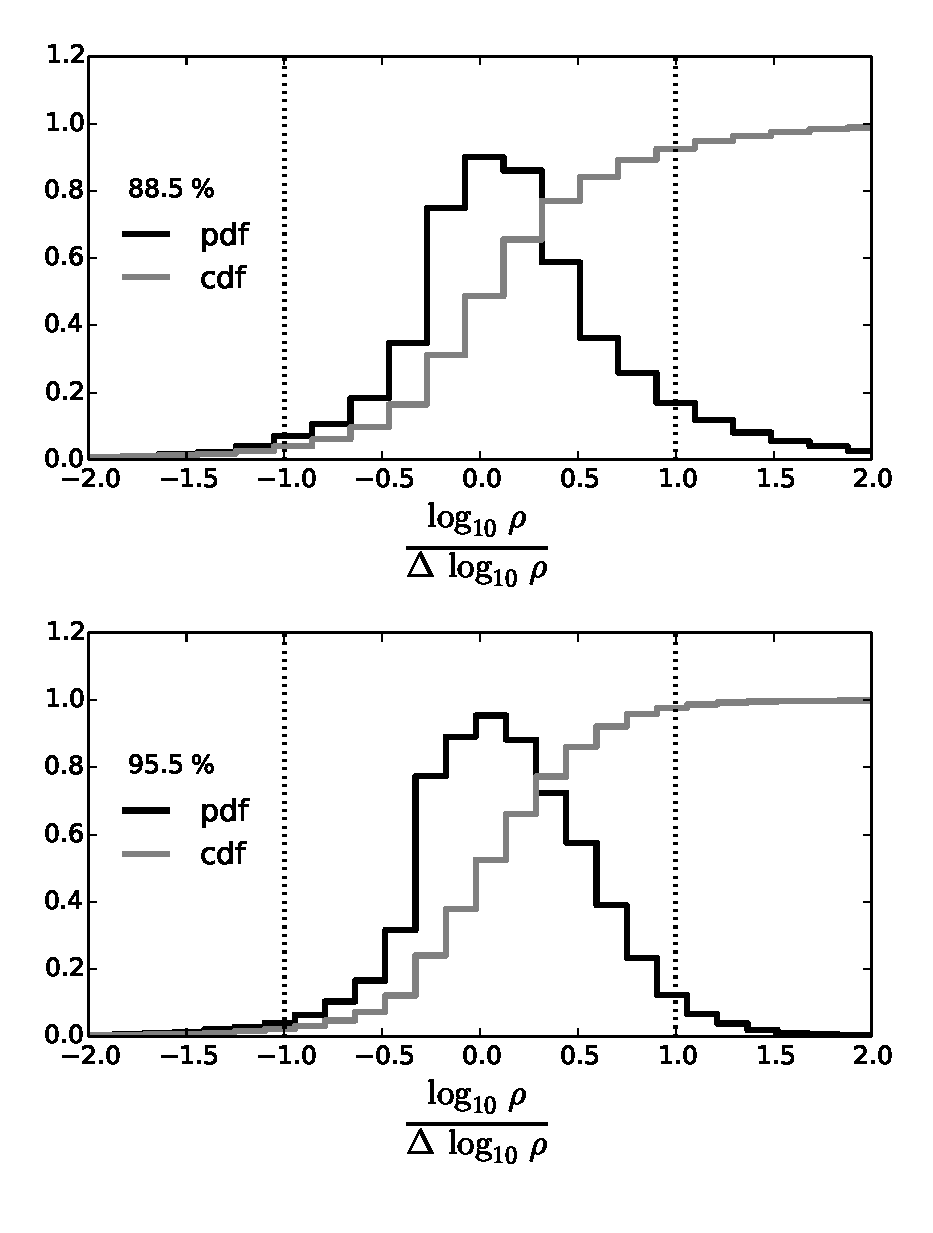
\includegraphics[width=\linewidth]{figures/v1_0/delta_array_histogram_wedge_sim_data_snr_log_ratio_0.3m_ground_custom_gaussian_FG_model_asm_all_sky_nside_64_Tsys_90.0K_185.0_MHz_30.7_MHz_bnw2.0.eps}
\caption{Significance of logarithm of ratio of observed to simulated visibilities relative to expected uncertainty restricted to the {\it foreground wedge} for the {\it off--zenith} (top) and {\it zenith} (bottom) pointings. Probability densities and cumulative distributions are shown in black and gray respectively. Region inside the dotted vertical lines denotes when the ratio, $\rho$, is consistent with unity subject to expected uncertainty. Also indicated in percentages are confidence levels estimated conservatively for such a consistency. They are $\sim$~90\% and $\sim$~95\% for {\it off--zenith} and {\it zenith} pointings respectively. \label{fig:data-sim-ratio-snr}}
\end{figure}

These uncertainties are presented only to confirm the qualitative agreement already seen between figures~\ref{fig:fhd_data} and \ref{fig:sim_data} and are not intended to serve as a comprehensive estimate of all uncertainties involved. However, since we have not accounted for numerous other uncertainties, especially in the data, such as uncertainties in the antenna power pattern, calibration, radio frequency interference (RFI), and wide field imaging effects, our estimates are conservative. Accounting for such uncertainties will only improve our confidence level in this comparison. Our primary objective is to explore in detail the foreground signatures embedded in the {\it foreground window}.

\section{Delay Spectrum Analysis}\label{sec:delay-spectrum-analysis}

Having established that results from modeling match those from data, we proceed to examine in further detail the signatures seen in the modeled delay spectra. 

A number of factors are responsible for the characteristics noted in the delay spectra obtained from data and through modeling. We address these factors below:
\begin{itemize}

\item {\it Sky Model}: Our model of the sky consists of bright compact sources and diffuse emission. Both of these kinds of emission are anisotropic and so is the resulting composite model. In fact, the pointing for MWA observations is chosen from regions of low foreground emission. In our study, we have divided the transiting sky into four different ``bow-tie'' shaped regions with equal areas and zenith as the origin. This results in the ability to attribute the features in the delay spectrum to eight different sectors of the sky.

\item {\it Baseline Orientation}: Since the spatial structure of our foreground model is not expected to be isotropic, we divide our interferometer baselines by their orientation ($\theta_\textrm{b}$) measured counter-clockwise from East. We use the following bins: $-67\fdg 5\le \theta_\textrm{b} < -22\fdg 5$, $-22\fdg 5\le \theta_\textrm{b} < 22\fdg 5$, $22\fdg 5\le \theta_\textrm{b} < 67\fdg 5$, and $67\fdg 5\le \theta_\textrm{b} < 112\fdg 5$. The bin centers are oriented towards South-East, East, North-East, and North respectively. 

\item {\it Tile Pointing and Power Pattern}: Since the MWA tiles are phased electronically, the power pattern of the tile changes in any observing mode that tracks the source. Our observations consist of a combination of allowing the sky to drift and tracking the sky. In our study, we take into account the effect of changing power pattern of the antennas on the delay spectrum. The LST of our data ranges from $\sim$~21 hours through $\sim$~2 hours (see figure~\ref{fig:pointings}). For comparisons, we choose two snapshot observations at LST of 22.08~hours (off--zenith pointing) and 0.09~hours (zenith pointing). 

\item {\it Instrumental Bandpass}: The instrumental bandpass characteristics have a direct effect on the delay transform owing to a Fourier relationship between the two. Due to excision of noisy edge channels repeated in each coarse channel of our bandpass, we see repeated patterns of the {\it foreground wedge} in the delay spectra. As already mentioned earlier, we have used the deconvolution algorithm ({\it CLEAN}) to rid the delay spectra of band shape effects. Since this paper focuses on studying the effects of foreground on the delay spectra, we do not pursue the characterization of artifacts from the band shape and imperfections in {\it CLEAN} deconvolution.

\end{itemize}

The signatures we henceforth identify in the delay spectrum are characterized as arising out of the aforementioned factors. Due to numerous combinations of such factors, we use unique codes for these combinations as described in table~\ref{tab:codes}. The first column refers to the place holder of the specific parameter in the code sequence from left to right. The parameter codes are specified in this order. The second column gives the parameter used in describing features in delay spectrum. The third column denotes the code describing the parameter. Snapshot index uniquely specifies the snapshot and carries a numeric code (1 and 2 for off-zenith and on-zenith snapshots respectively) leading the code sequence. Following this, the type of emission is specified as compact, diffuse, Galactic center, or Galactic plane using codes C, D, GC, or GP respectively. Although in reality, a feature could be due to a combination of emission types, the code we use refers to the predominant type of emission that can be attributed to the feature. The next code specifies the direction of this predominant source of emission. The code values for the direction of emission are the usual abbreviations of the cardinal and ordinal directions besides Z (zenith). Following this is the code for the baseline orientation bin in the half-plane specified as S, SE, E, and NE along directions south, south-east, east, and north-east respectively. Code `A' is used to refer to all baselines. Finally, the parameter describing the region of antenna power pattern coincident with the predominant emission responsible for the feature is specified as P (primary lobe) and S (secondary lobe). The secondary lobe code carries a numeral suffix to further specify uniquely the sidelobe in the direction of emission. For example, a feature code 1-D-W-E-P indicates it is from the first snapshot (1) arising due to diffuse emission (D) westward (W) of zenith observed by predominantly eastward (E) baselines centered on the primary beam (P) of the antenna power pattern. Simiarly, feature code 2-GC-W-NE-S3 implies the feature is seen in the second snapshot (2) due to the Galactic Center (GC) that is westward (W) of zenith by north-eastward (NE) baselines and the region coincides with the third sidelobe (S3) in the direction of emission.

\begin{table*}[htp]
\caption[]{Codes used to describe signatures in delay spectrum.\label{tab:codes}}
\centering
\begin{tabular}{ccc}
\tableline\tableline\tableline
Order & Parameter Description & Code \\
\tableline\tableline
1 & Snapshot index & 1, 2, \ldots \\
2 & Type of emission & C (compact), D (diffuse), GC (Galactic center), GP (Galactic plane) \\
3 & Direction of emission & E (east), N (north), W (west), S (south), Z (zenith)\\
& & NE (north-east), NW (north-west), SW (south-west), SE (south-east) \\
4 & Baseline orientation & E (east), S (south), SE (south-east), NE (north-east), A (all) \\
5 & Region in antenna power pattern & P (primary beam), Sn ($n$-th sidelobe, $n=1,2,\ldots$)\\
& (in the direction of emission) & \\
\tableline
\end{tabular}
\end{table*}

We wish to note that numerous features overlap at varying levels of significance as a result of various combiantions of parameters. We assign the features to their predominant causes. Secondly, we have used noiseless cases to clearly illustrate the observed foreground signatures. With the addition of noise in the visibilities which is subject to observing time, some of the weaker features may not be as prominently visible. 

\subsection{Diffuse Foregrounds}\label{sec:diffuse}

Figure~\ref{fig:dsm} shows the noiseless delay spectra due to diffuse emission. Figure~\ref{fig:dsm_delay_spectrum_snap0} and \ref{fig:dsm_delay_spectrum_snap1} correspond to off-zenith and on-zenith snapshots respectively. In general, shorter baselines are expected to be receptive to large scales such as from diffuse emission as well as from small scales from compact objects. This effect is most clearly visible in the on-zenith snapshot noted by feature code 2-D-Z-A-P which stands for the signature observed due to diffuse emission from zenith direction on short baselines of all orientations restricted primarily to the primary beam. This is a notable feature on baselines of length $\lesssim 60$~m. For a frequency of 185~MHz, this length scale corresponds to angular scales of $\gtrsim 1\fdg 5$ on the sky. This feature is noted only for diffuse emission from inside the primary beam.

The most prominent feature, however, is 1-GC-W-E-S3 in figure~\ref{fig:dsm_delay_spectrum_snap0}. This is noted in the off-zenith snapshot caused by the bright Galactic center which is on the west at an altitude of $\sim 33$\arcdeg with $\sim 100$~minutes remaining before it sets. This emission is observed as it is coincident with the third sidelobe of the power pattern in the westward direction with a neagtive delay of value almost close to the horizon limit on eastward baselines.

\begin{figure*}[htp]
\centering
\subfloat[][Off-zenith delay spectra from diffuse foreground model]{\label{fig:dsm_delay_spectrum_snap0}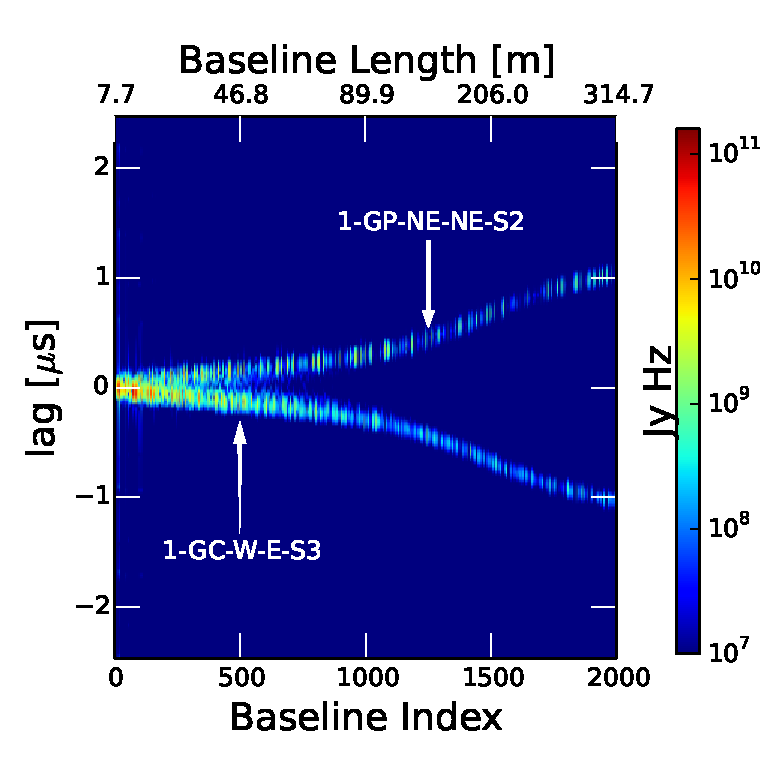
\includegraphics[width=0.49\linewidth]{figures/v1_0/annotated_combined_baseline_noiseless_CLEAN_visibilities_custom_FG_model_dsm_all_sky_nside_128_185.0_MHz_30.7_MHz_bnw2.0_snap_0.eps}}
\subfloat[][On-zenith delay spectra from diffuse foreground model]{\label{fig:dsm_delay_spectrum_snap1}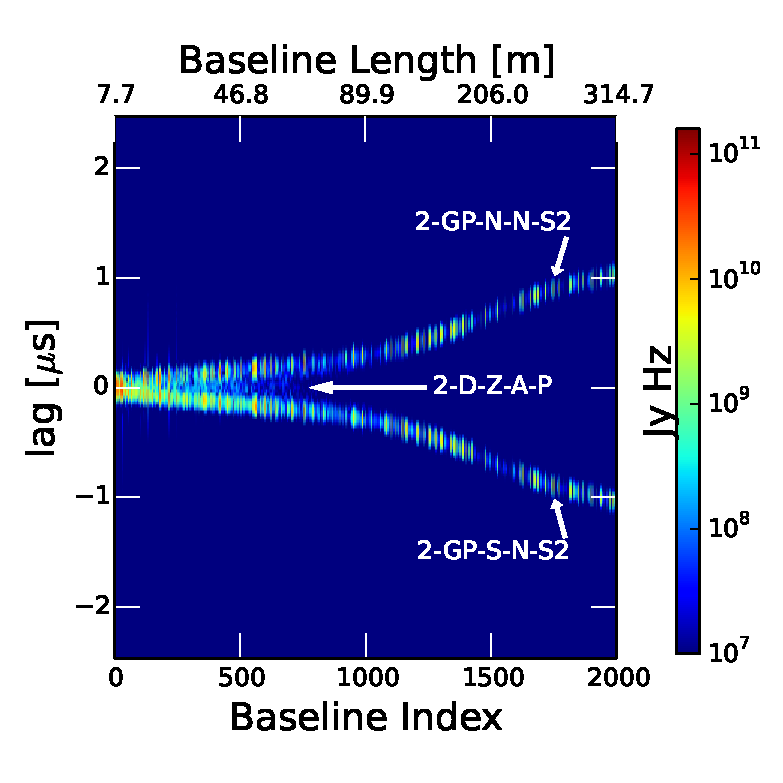
\includegraphics[width=0.49\linewidth]{figures/v1_0/annotated_combined_baseline_noiseless_CLEAN_visibilities_custom_FG_model_dsm_all_sky_nside_128_185.0_MHz_30.7_MHz_bnw2.0_snap_1.eps}}\\
\caption{Delay spectrum visibility amplitudes (in units of Jy~Hz) from diffuse foreground emission obtained on baselines of length $\lesssim 314.7$~m. The left and right panels correspond to off-zenith and on-zenith snapshots respectively. These are noiseless delay spectra obtained after {\it CLEAN} deconvolution along delay axis. A logarithmic color scale is used. Most prominent features are due to the bright Galactic center shining through the third sidelobe (1-GC-W-E-S3), diffuse emission of short baselines at zero delays (2-D-Z-A-P), and diffuse emission on long baselines close to the horizon limit leaking in through the second sidelobes (1-GP-NE-NE-S2, 2-GP-N-N-S2, and 2-GP-S-N-S2). Features from diffuse emission are predominantly edge-heavy resembling a two-pronged fork. See text for a detailed description of these features.}
\label{fig:dsm}
\end{figure*}

\subsubsection{Diffuse Emission On Long Baselines }\label{sec:fork}

Interestingly, in contrast to feature code 2-D-Z-A-P, all the other features in figures~\ref{fig:dsm_delay_spectrum_snap0} and \ref{fig:dsm_delay_spectrum_snap1} extend from the shortest ($\sim 7.7$~m) to longest baselines ($\sim 314.7$~m). We argue this is because even longer baselines are shortened when projected against directions along the baseline vector towards the horizon while considering an all-sky foreground model. Such a shortening due to projection effects allows diffuse emission from close to the horizon to be observed at maximum delays that correspond to the horizon limit even on long baselines. Feature 1-GP-NE-NE-S2 in figure~\ref{fig:dsm_delay_spectrum_snap0}, and features 2-GP-N-N-S2 and 2-GP-S-N-S2 in figure~\ref{fig:dsm_delay_spectrum_snap0} demonstrate this effect of shortening of baselines. 1-GP-NE-NE-S2 corresponds to emission observed from the Galactic plane from north-eastward directions by north-eastward baselines from the second sidelobe in their power pattern. Features 2-GP-N-N-S2 and 2-GP-S-N-S2 are also Galactic plane emission from southward and northward directions observed by second sidelobes of northward baselines with opposite delays. Owing to their apparent structure in delay spectra, we hereafter refer broadly to this edge-heavy structure as the ``two-pronged fork'' feature. 

Thus, the most notable features from diffuse emission are those from primary beam area on short baselines, bright Galactic center from the third sidelobe, and the two-pronged fork.

\subsection{Compact Foregrounds}\label{sec:compact}

Figure~\ref{fig:csm} shows the noiseless delay spectra obtained from compact foreground objects. The off-zenith and on-zenith snapshot delay spectra are shown in figures~\ref{fig:csm_delay_spectrum_snap0} and \ref{fig:csm_delay_spectrum_snap1} respectively. 

In the off-zenith snapshot, the most prominent feature 1-C-E-E-P arises due to eastward baselines observing the eastward sky at positive delays centered on the primary beam. The next prominent feature 1-C-E-N-P at zero delays arises due to the compact emission from eastward sky centered on the primary beam observed by northward baselines. Features 1-C-NE-NE-S2 and 1-C-W-E-S3 at positive and negative horizon limits are caused by north-eastward sky emission observed by the second sidelobe of north-eastward baselines and westward sky centered on the third sidelobe of eastward baselines respectively. 

The most prominent feature in the on-zenith snapshot is 2-C-Z-A-P appearing at zero delays caused by compact sources at zenith observed by all baselines along their primary beams. First and second sidelobes along north and south observed by northward baselines contribute to symmetric positive and negative delays as demonstrated by features 2-C-S-N-S1, 2-C-N-N-S1, 2-C-S-N-S2, and 2-C-N-N-S2.

\begin{figure*}[htp]
\centering
\subfloat[][Off-zenith delay spectra from compact foreground objects]{\label{fig:csm_delay_spectrum_snap0}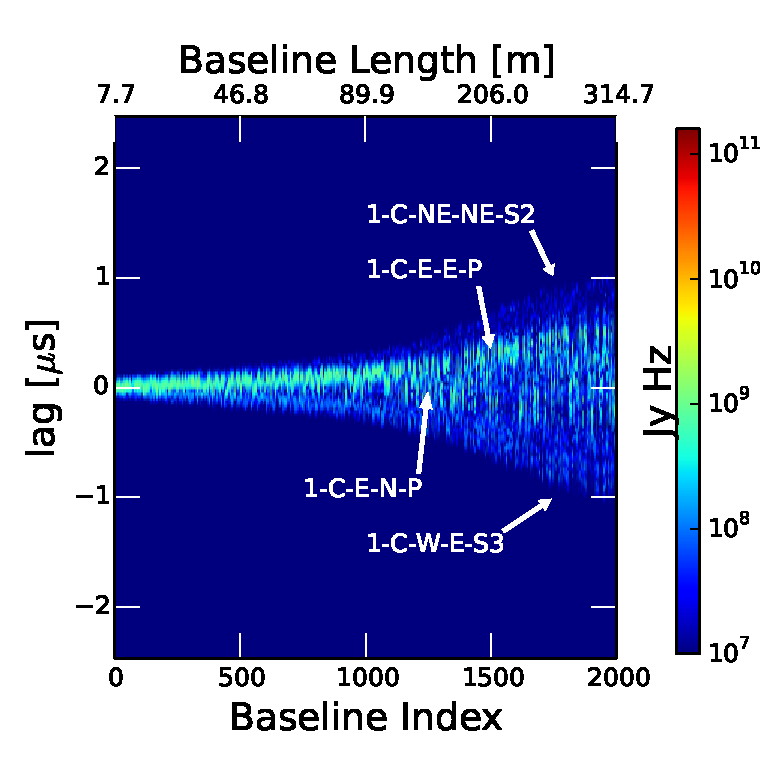
\includegraphics[width=0.49\linewidth]{figures/v1_0/annotated_combined_baseline_noiseless_CLEAN_visibilities_custom_FG_model_csm_all_sky_nside_128_185.0_MHz_30.7_MHz_bnw2.0_snap_0.eps}}
\subfloat[][On-zenith delay spectra from compact foreground objects]{\label{fig:csm_delay_spectrum_snap1}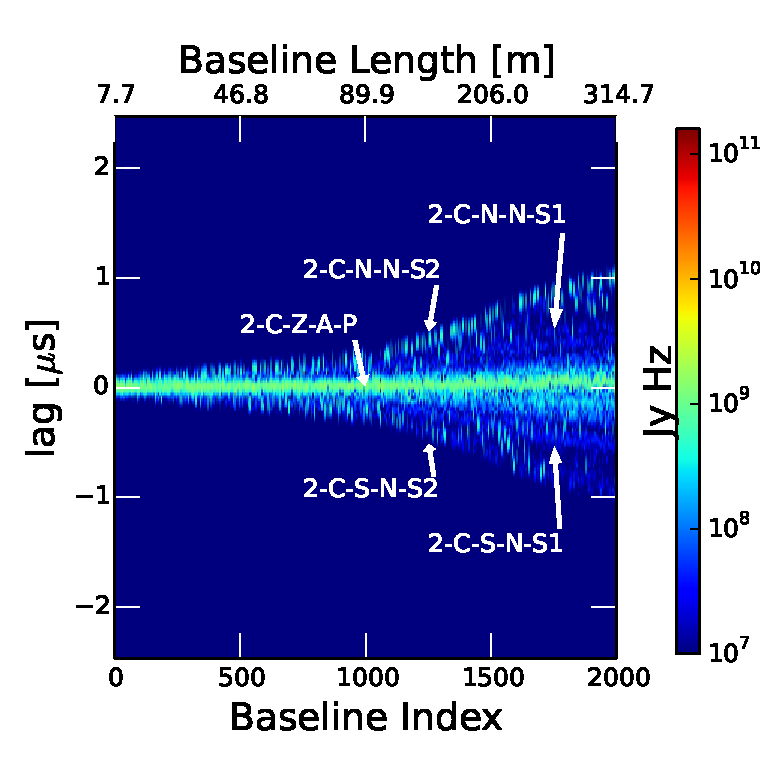
\includegraphics[width=0.49\linewidth]{figures/v1_0/annotated_combined_baseline_noiseless_CLEAN_visibilities_custom_FG_model_csm_all_sky_nside_128_185.0_MHz_30.7_MHz_bnw2.0_snap_1.eps}}\\
\caption{Same as figure~\ref{fig:dsm} but for compact foreground objects. Color scale is the same as in figure~\ref{fig:dsm}. The different features annotated are a result of emission observed by compact foreground objects through primary beam and sidelobes. Broadly, signatures in delay spectra of compact foreground objects are center-heavy in appearance. See text for a detailed description of the different features.}
\label{fig:csm}
\end{figure*}

While compact foreground objects give rise to features throughout the foreground wedge, the primary distinction between delay spectra of compact and diffuse foregrounds is that the latter are predominantly center-heavy when compared to edge-heavy features of the former. 

% Figure~\ref{fig:obs-begin} shows the delay spectra obtained with the compact foreground model described in \S\ref{sec:CSM} at the beginning of the observation when the MWA tiles are phased to point at RA = 4\fdg 387, Dec = -29\fdg 86. The contours of the antenna power pattern are shown in the central panel. The flux densities of compact foreground objects multiplied by the antenna power pattern at the respective locations are shown on a logarithmic color scale right below the central panel. For reference, maps of delays between the received signals are shown for 100~m baselines with $\theta_b=0\arcdeg, 45\arcdeg, 90\arcdeg, \textrm{and}\,135\arcdeg$ to relate the strength of emission with the corresponding delay in the delay spectra. 

% \begin{figure*}[htb]
% \centering
% % \subfloat[][Delay spectra at the beginning of observation]{\label{fig:SNR1D_6hrs_167_single_e0}\includegraphics[width=\linewidth]{}}
% 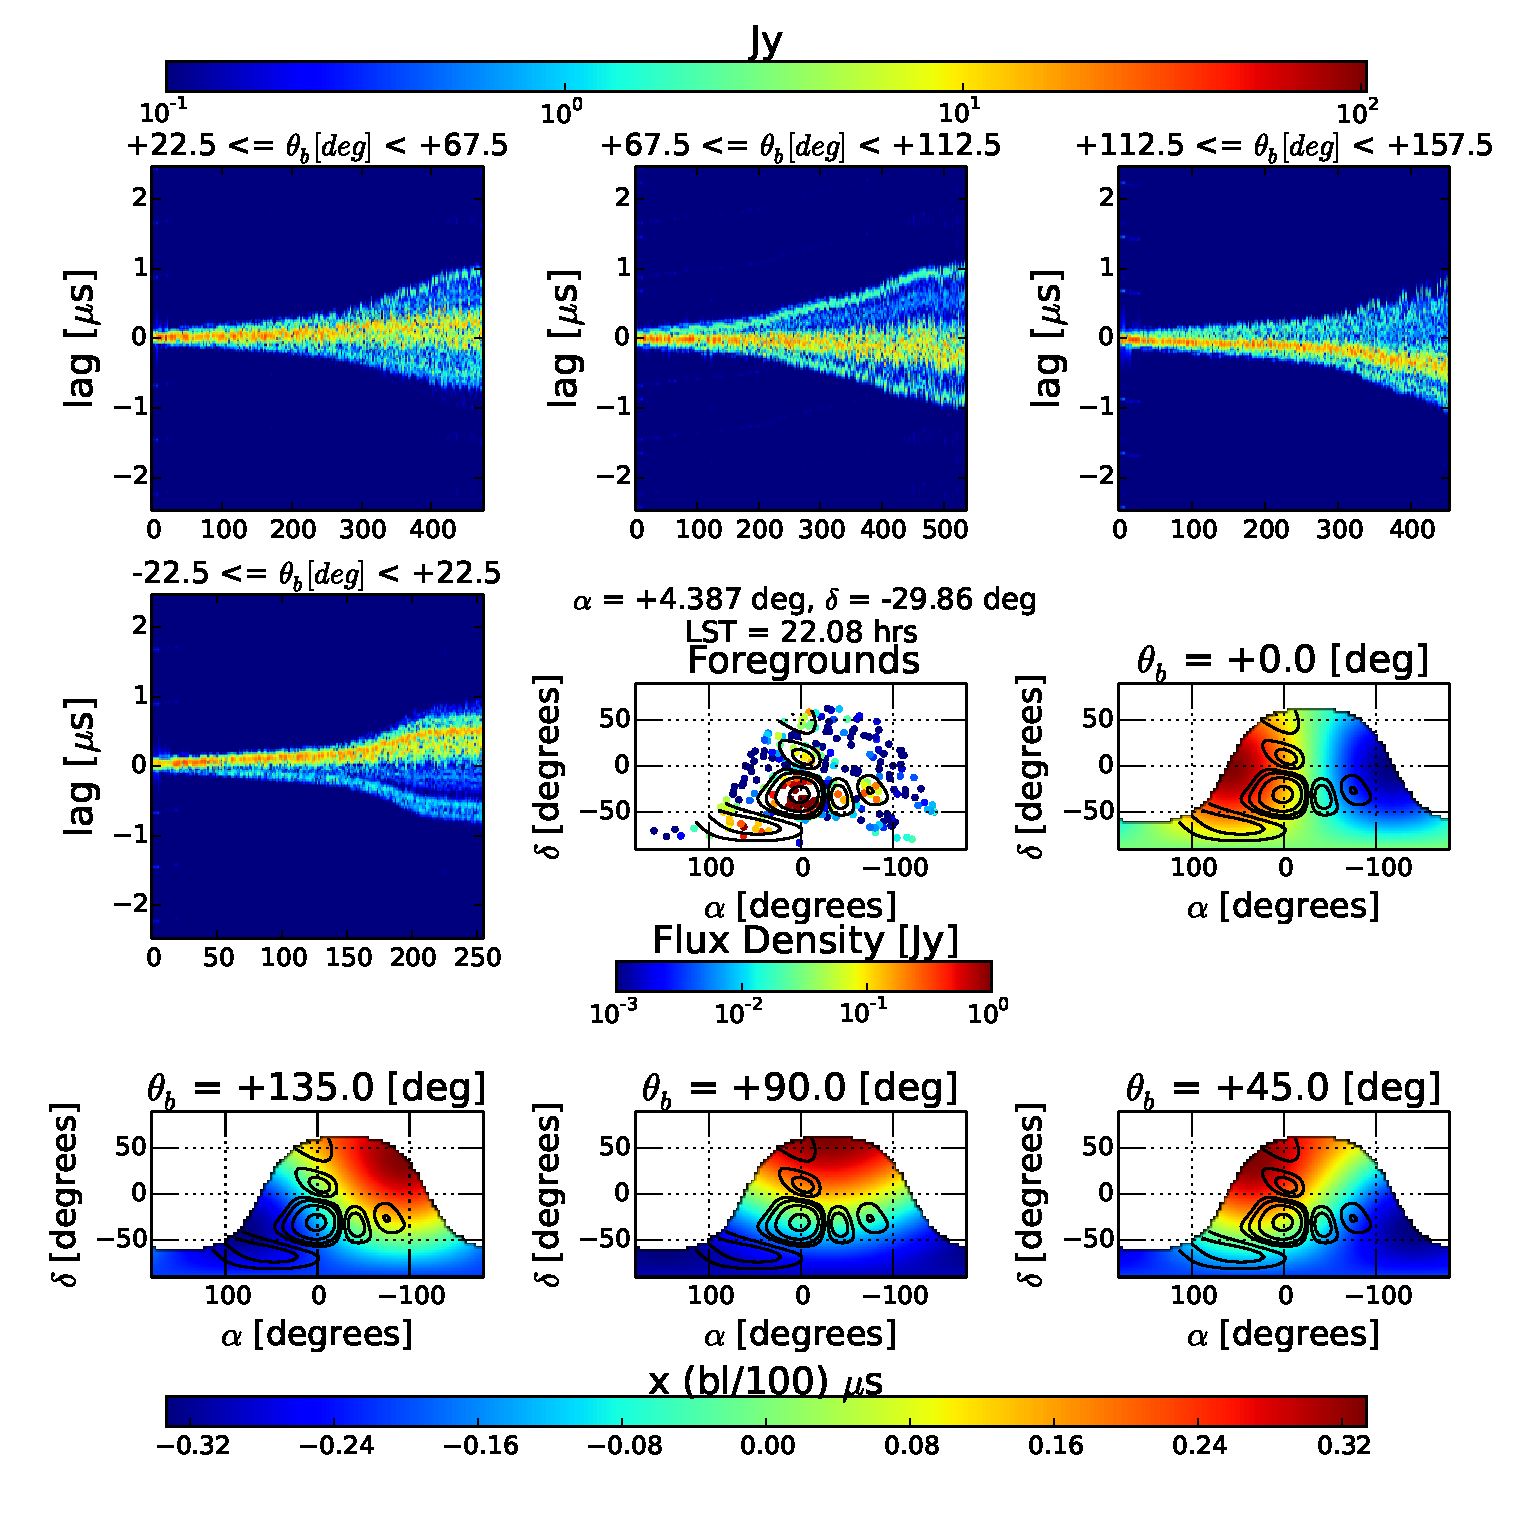
\includegraphics[width=\linewidth]{figures/v1_0/multi_baseline_CLEAN_visibilities_custom_gaussian_FG_model_csm_all_sky_nside_128_30.7_MHz_bnw2.0_snapshot_0.eps}
% \caption{Delay spectra, compact foreground sources, and delay maps for a snapshot at the beginning of the observation pointed at RA = 4\fdg 387, Dec = -29\fdg 86 at LST = 22.08 hours. The phase center is at RA = -28\fdg 8, Dec = -26\fdg 701. The baselines have been binned by their orientation ($\theta_\textrm{b}$) anti-clockwise from east. The center-right panel shows delay spectra from baselines oriented between -22\fdg 5 $\le \theta_\textrm{b}<$+22\fdg 5. The upper-right, upper-center, and upper-left panels have baseline orientations lying between +22\fdg 5 $\le \theta_\textrm{b}<$+67\fdg 5, +67\fdg 5 $\le \theta_\textrm{b}<$+112\fdg 5, and +112\fdg 5 $\le \theta_\textrm{b}<$+157\fdg 5, respectively. The color scale in these delay spectra are given by the color bar on top. The panels diametrically opposite to aforementioned panels represent the delay map on the sky for a 100~m baseline oriented along east, north-east, north, and north-west respectively. The color scale for these delay maps is specified at the bottom. Delays are positive towards east and north sky positions for eastward and northward baseline orientations respectively. The central panel shows the compact foreground model multiplied by the antenna power pattern. The color scale is specified below the panel. Also shown are contours of the antenna power pattern. The contour levels shown are: 0.0078125, 0.03125, 0.125, and 0.5.}
% \label{fig:obs-begin}
% \end{figure*}

% \begin{figure*}[htb]
% \centering
% % \subfloat[][Delay spectra at the beginning of observation]{\label{fig:SNR1D_6hrs_167_single_e0}\includegraphics[width=\linewidth]{}}
% 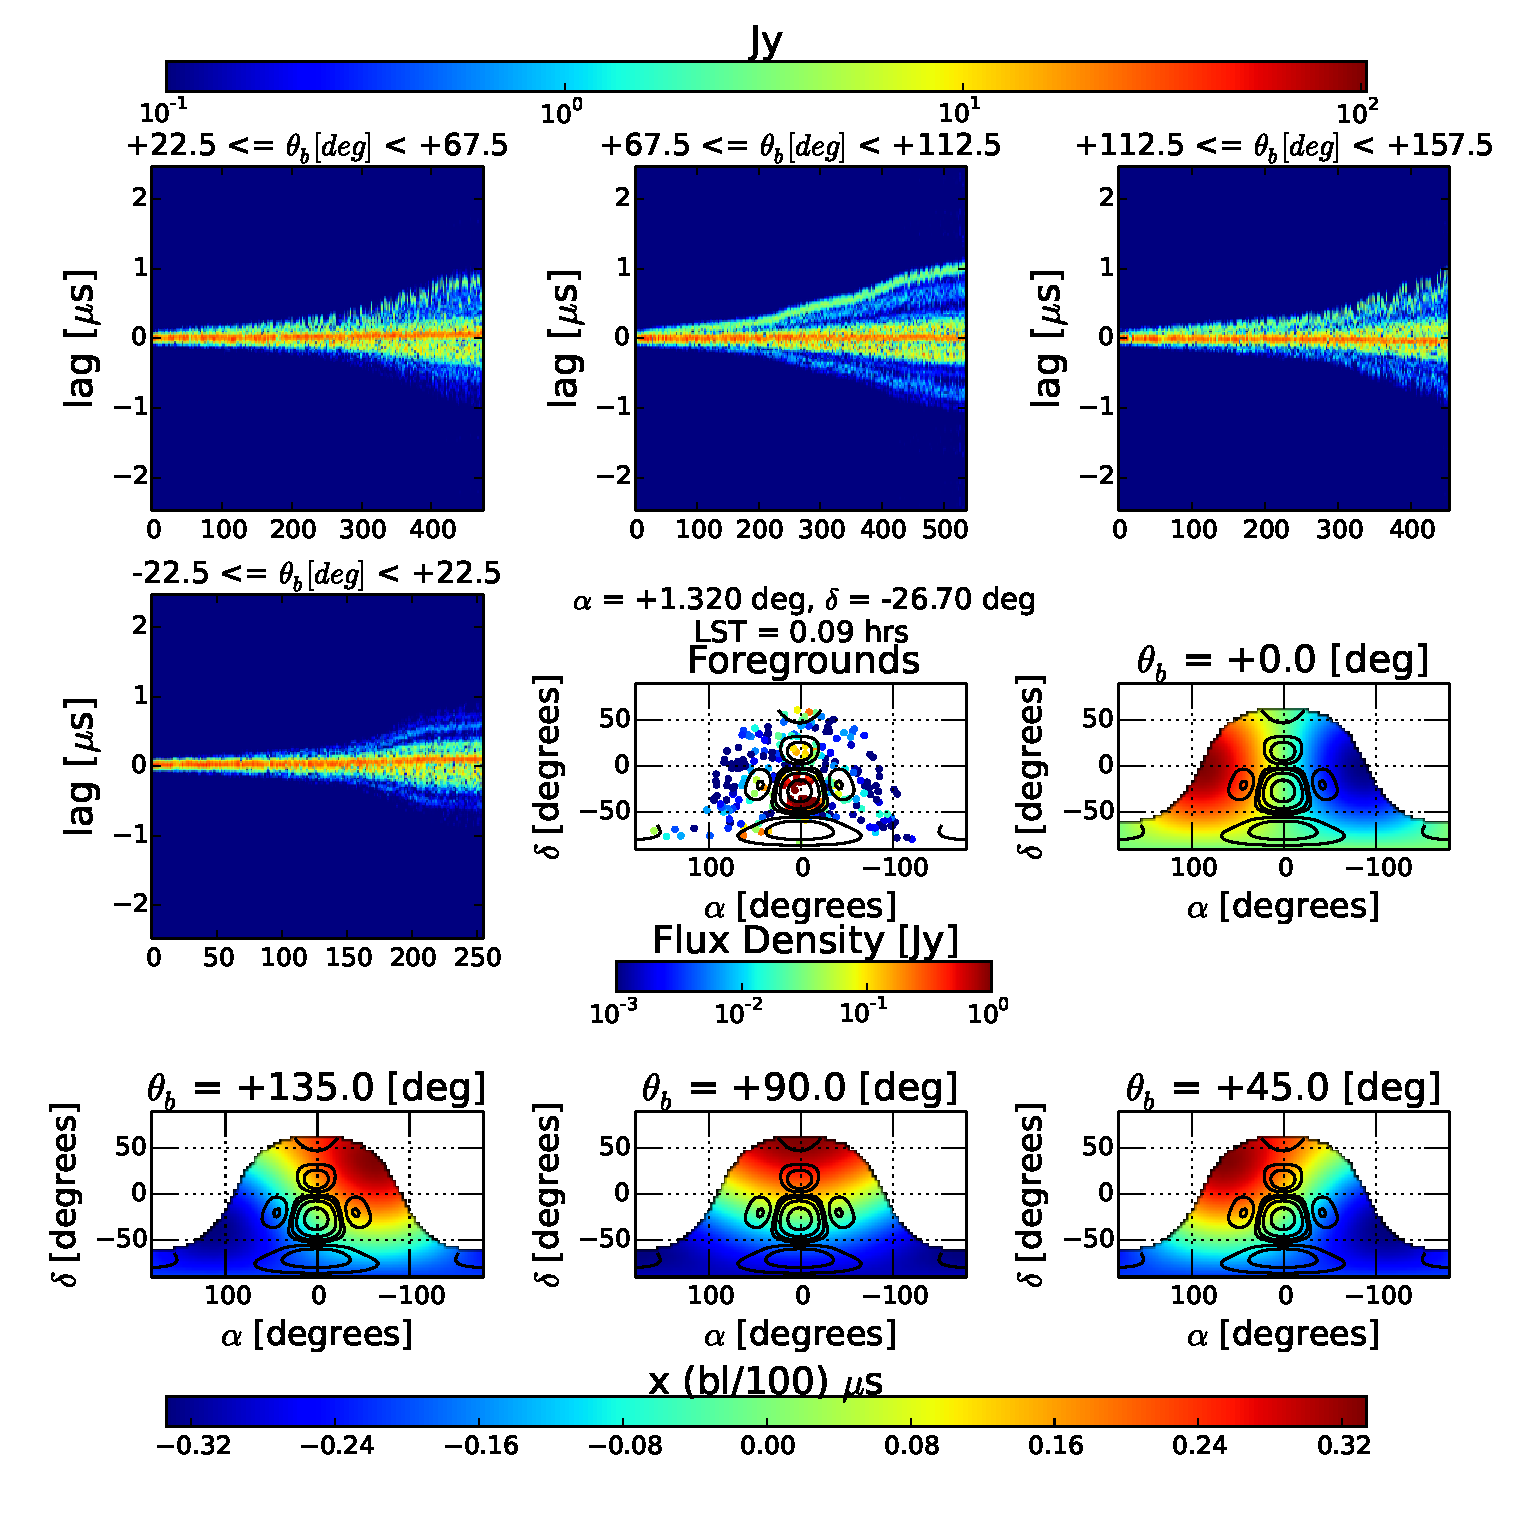
\includegraphics[width=\linewidth]{figures/v1_0/multi_baseline_CLEAN_visibilities_custom_gaussian_FG_model_csm_all_sky_nside_128_30.7_MHz_bnw2.0_snapshot_1.eps}
% \caption{Same as figure~\ref{fig:obs-begin} but for a snapshot during the middle of the observation pointed at RA = +1\fdg 320, Dec = -26\fdg 70 at LST = 0.09 hours. The phase center is at RA = 1\fdg 35, Dec = -26\fdg 701. }
% \label{fig:obs-middle}
% \end{figure*}

\subsection{All-Sky Composite Foreground Model}\label{sec:composite}

Delay spectra from the all-sky foreground model in our study display a composite feature set drawn from the features of compact and diffuse foreground models. Figures~\ref{fig:asm_delay_spectrum_snap0} and \ref{fig:asm_delay_spectrum_snap1} show the delay spectra for the composite all-sky foreground model. While features from both its constituents occupy and overlap in different regions of the foreground wedge, their relatives magnitudes determine the resultant signatures seen in the delay spectra. For instance, the fork-shaped features of diffuse emission are brighter by a factor $\gtrsim 10$ relative to the compact foreground features at the edges of delay spectra in the respective snapshots. Hence, features 1-C-W-E-S3 and 1-C-NE-NE-S2 in figure~\ref{fig:csm_delay_spectrum_snap0} have been masked by features 1-GC-W-E-S3 and 1-GP-NE-NE-S2 respecively from diffuse emission in figure~\ref{fig:dsm_delay_spectrum_snap0}. Similarly, the edge features 2-C-S-N-S2 and 2-C-N-N-S2 from compact objects in figure~\ref{fig:csm_delay_spectrum_snap1} have been masked by diffuse emission features 2-GP-S-N-S2 and 2-GP-N-N-S2 respectively in figure~\ref{fig:dsm_delay_spectrum_snap1}.

On the other hand, in central and inner regions of the wedge, clearly the center-heavy compact foreground model features dominate by $\gtrsim 2$ orders of magnitude relative to features arising out of diffuse emission. This is quite evident since almost all the diffuse emission features are confined to the edges of the wedge. Further, 2-D-Z-A-P in figure~\ref{fig:dsm_delay_spectrum_snap1} is completely masked by 2-C-Z-A-P in figure~\ref{fig:csm_delay_spectrum_snap1}. Thus the inner regions of the wedge consist only of compact foreground features 1-C-E-N-P and 1-C-E-E-P in figure~\ref{fig:asm_delay_spectrum_snap0} and 2-C-Z-A-P, 2-C-S-N-S1 and 2-C-N-N-S1 in figure~\ref{fig:asm_delay_spectrum_snap1}.

Figures~\ref{fig:baseline_composite_asm_delay_spectrum_snap0} and \ref{fig:baseline_composite_asm_delay_spectrum_snap1} show the delay spectra from the diffuse and compact foreground models as well as from the composite model for the off-zenith and on-zenith snapshots respectively for a selected baseline labeled as ``155-154''. This baseline is of length $\simeq 201$~m and orientation $\theta_b\simeq 13\fdg 7$. These are effectively vertical slices of figures~\ref{fig:asm_delay_spectrum_snap0} and \ref{fig:asm_delay_spectrum_snap1} through the baseline location. The horizon delay limits are shown by vertical gray lines. Diffuse emission is negligible in the off-zenith snapshot except at the negative horizon delay limit. This is identified to be feature 1-GC-W-E-S3 noted in figure~\ref{fig:asm_delay_spectrum_snap0} due to the bright Galactic center on the westward sky observed by eastward baseline through its third sidelobe. All the other features are predominantly due to compact foreground objects. The peak at delay of $\sim 0.3\,\mu$~s is identified as feature 1-C-E-E-P in figure~\ref{fig:asm_delay_spectrum_snap0}. The peak at zero delay is from feature 1-C-Z-A-S1 while the other secondary peaks arise compact sources coincident with sidelobes of the power pattern. In the on-zenith snapshot, the feature 1-C-E-E-P has transformed to feature 2-C-Z-A-P due to change in pointing position. The diffuse emission is confined to the edges labeled by features 2-D-W-E-S2 and 2-D-E-E-S2. All intermediate peaks are due to compact foreground objects observed through the different sidelobes of the antenna power pattern. 

\begin{figure*}[htp]
\centering
\subfloat[][Off-zenith delay spectra from composite foreground model]{\label{fig:asm_delay_spectrum_snap0}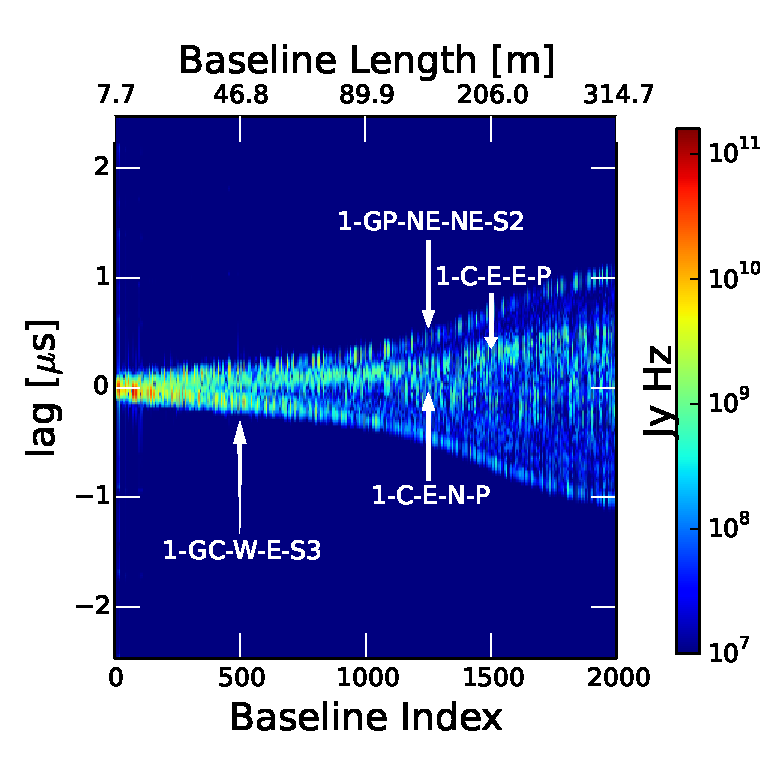
\includegraphics[width=0.49\linewidth]{figures/v1_0/annotated_combined_baseline_noiseless_CLEAN_visibilities_custom_FG_model_asm_all_sky_nside_128_185.0_MHz_30.7_MHz_bnw2.0_snap_0.eps}}
\subfloat[][Off-zenith delay spectra from composite foreground model]{\label{fig:asm_delay_spectrum_snap1}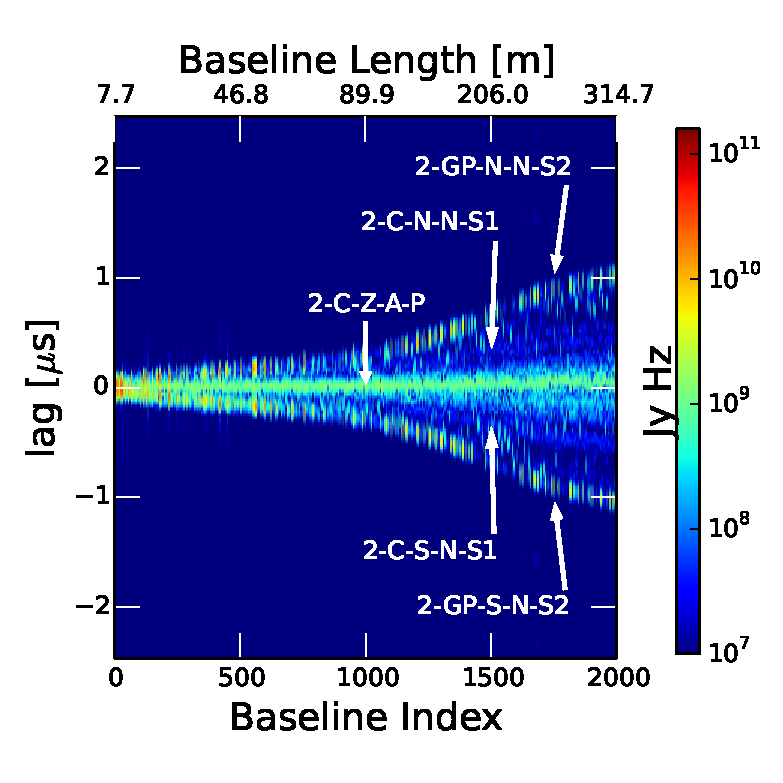
\includegraphics[width=0.49\linewidth]{figures/v1_0/annotated_combined_baseline_noiseless_CLEAN_visibilities_custom_FG_model_asm_all_sky_nside_128_185.0_MHz_30.7_MHz_bnw2.0_snap_1.eps}}\\
\subfloat[][Off-zenith composite delay spectrum on eastward baseline]{\label{fig:baseline_composite_asm_delay_spectrum_snap0}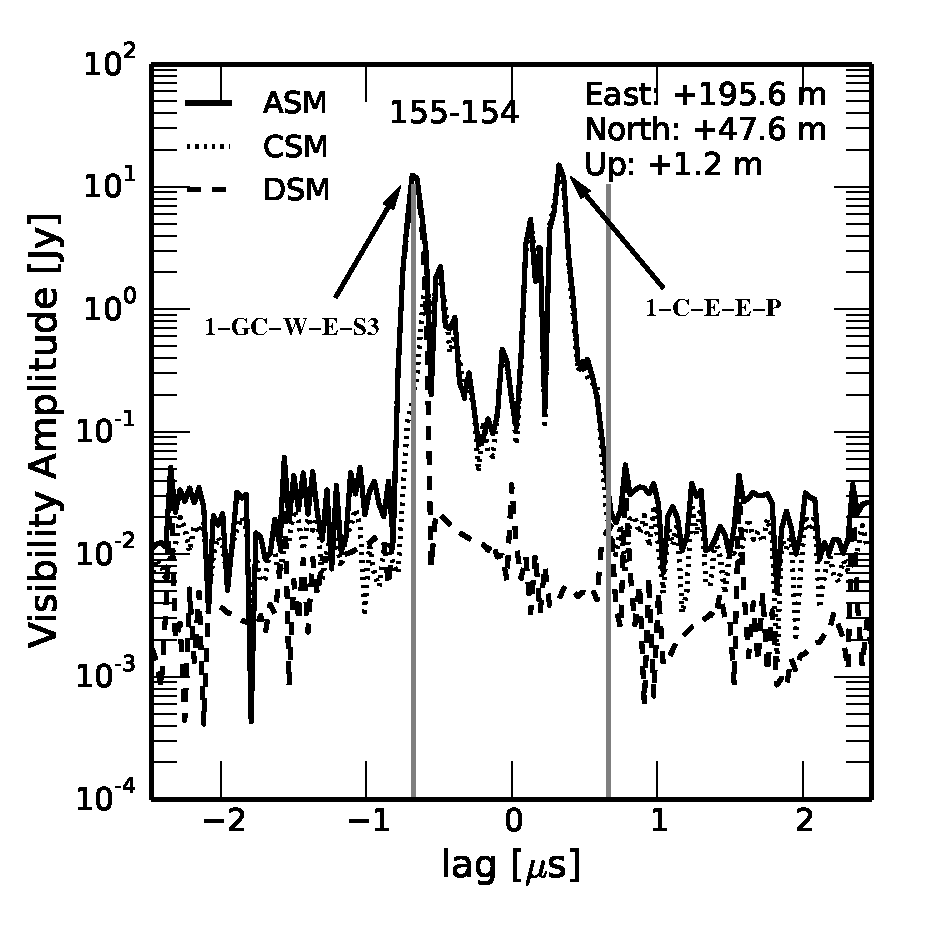
\includegraphics[width=0.49\linewidth]{figures/v1_0/baseline_155-154_composite_noiseless_delay_spectrum_snapshot_0.edited.eps}}
\subfloat[][On-zenith composite delay spectrum on eastward baseline]{\label{fig:baseline_composite_asm_delay_spectrum_snap1}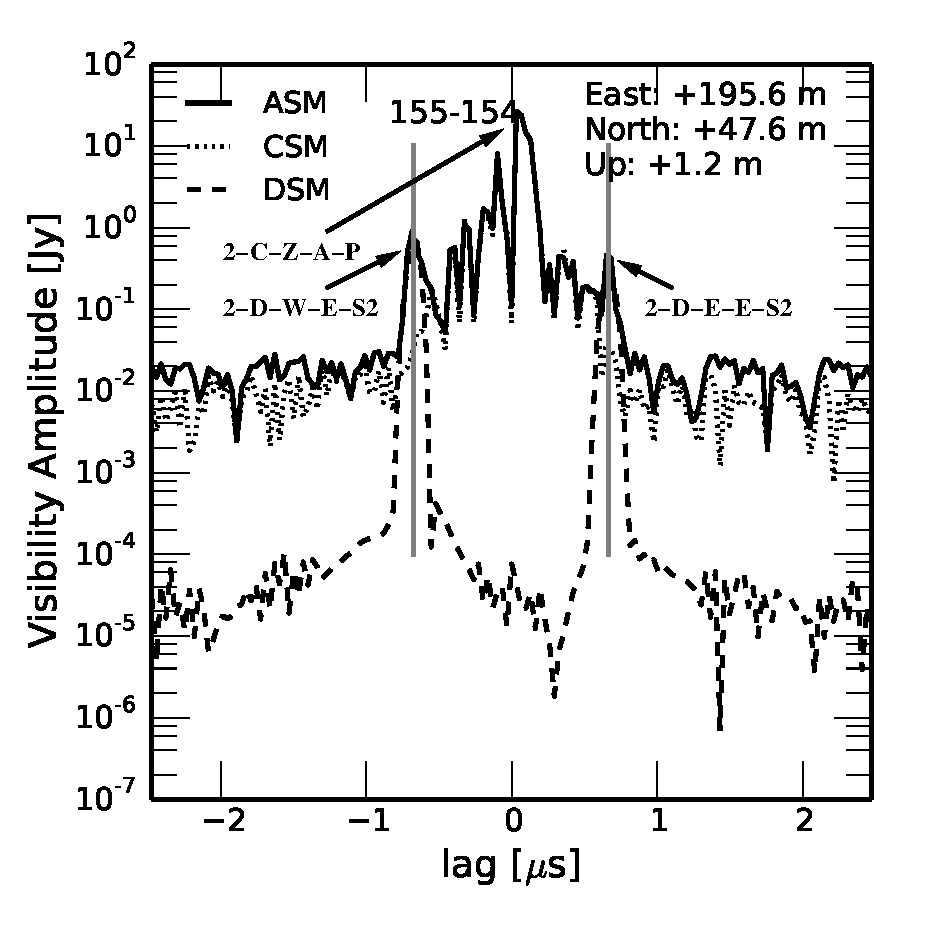
\includegraphics[width=0.49\linewidth]{figures/v1_0/baseline_155-154_composite_noiseless_delay_spectrum_snapshot_1.edited.eps}}\\
\caption{{\it Top}: Same as figure~\ref{fig:dsm} but for a composite all-sky foreground model consisting of both diffuse emission and compact objects. The color scale used is the same. The different features annotated arise from those in figures~\ref{fig:dsm} and \ref{fig:csm}. Inner regions of the wedge are dominated by center-heavy features such as 1-C-E-N-P, 1-C-E-E-P, 2-C-Z-A-P, 2-C-N-N-S1 and 2-C-S-N-S1 characteristic of compact objects. Outer regions are dominated by edge-heavy fork-shaped features such as 1-GC-W-E-S3, 1-GP-NE-NE-S2, 2-GP-S-N-S2 and 2-GP-N-N-S2 characteristic of diffuse emission. The resultant structure in delay spectrum takes the form of a {\it pitchfork}. {\it Bottom}: Slices of delay spectrum visibility amplitudes from the top panel at the location of a selected eastward baseline. The baseline vector is $\sim 201$~m in length oriented $\sim 13\fdg 7$ measured anti-clockwise from east. The foreground components are: diffuse sky model (DSM, dashed lines), sky made of compact sources (CSM, dotted lines) and all-sky composite model (ASM, solid lines). The gray vertical lines signify the wedge boundaries set by the horizon delay limit. Compact sources dominate the delay spectra in the inner part of the wedge as marked by features 1-C-E-E-P and 2-C-Z-A-P. Edge-heavy fork-shaped features such as 1-GC-W-E-S3, 2-D-W-E-S2 and 2-D-E-E-S2 from diffuse emission are more significant at the edges of the wedge. These give rise to a ``pitchfork'' appearance. Other secondary peaks inside the wedge are due to compact objects observed through sidelobes of the antenna power pattern. The secondary bumps outside the wedge in all the model components is a result of imperfect deconvolution along delay axis. Refer to text for detailed description of these features.}
\label{fig:asm}
\end{figure*}

Thus the composite all-sky foreground model results in a delay spectrum structure that captures both the edge-heavy two-pronged fork structure from diffuse foreground emission and the center-heavy features from compact foreground objects. Hereafter, we refer to this structure as a ``three-pronged pitchfork''. 

\section{Foreground Grading Diagnostic For Observations}\label{sec:fg-grading}



% \section{Discussion}\label{sec:discussion}

\section{Summary}\label{sec:summary}

Our primary motivation in this work is to analyze the signatures of foreground components in the measured delay spectrum. Such an analysis will be helpful in extending our knowledge on the challenge posed by foregrounds in studying the EoR and in devising techniques to mitigate EoR signal contamination from foregrounds. This is one of the first studies that uses an all-sky foreground model to study the resultant signatures on EoR delay spectrum.

Using parameters that match the instrument and EoR observations using the MWA, and an all-sky foreground model that consists of diffuse emission on scales $\gtrsim 0\fdg 85$ and bright compact sources from the NVSS and SUMSS catalogs, we model delay spectra obtained with the MWA on each of its baselines of length $\lesssim 315$~m. We confirm that the modeled delay spectra match the data obtained with the MWA. A wedge shaped structure is clearly noted as predicted by previous studies.

We use our simulations in a noiseless scenario to understand many of the foreground signatures seen in the delay spectra. We find that the delay spectra depend on observing parameters such as antenna pointing and LST, instrument parameters such as antenna power pattern and bandpass shape, and foreground parameters such as the nature of emission, spectral index, etc. A {\it CLEAN} deconvolution in delay-space was applied to remove the contaminating harmonic effects of frequency flagging. 

Notable features caused by diffuse emission include the bright Galactic center at the edge of the horizon to be observed through the far sidelobe of the antenna power pattern. As expected, diffuse emission in the primary beam of the antenna power pattern is present on short baselines of length $\lesssim 60$~m. Quite surprisingly, diffuse emission also leaves its footprint on long baselines on either side of the delay axis at the horizon delay limits. This clearly indicates that long baselines appear to be shortened in the direction of the horizon along the baseline vector and these short projected baselines are responsive to large scale diffuse emission. Thus, one of the most important findings of this study is the response of even long baselines to diffuse structures. The characteristic signature of diffuse emission appears to be a roughly symmetric edge-heavy feature taking the form of a {\it two-pronged fork}. 

On the other hand, compact foreground objects predominantly map onto inner regions of the wedge. Features arising from compact sources coincident with primary beam and sidelobes of antenna power pattern are clearly noted. In general, compact objects produce delay spectrum signatures that are center-heavy, in stark contrast to those from diffuse foregrounds.

A composite all-sky foreground model consisting of diffuse and compact foregrounds gives rise to a combination of edge-heavy fork shaped features from diffuse foregrounds and center-heavy features from compact foreground objects in the delay spectrum. The compact foreground features are brighter by $\gtrsim 3$ orders of magnitude brighter than the diffuse foreground features in the central regions of delay spectrum. On the other hand, the edge-heavy diffuse foreground features in the delay spectrum are $\gtrsim 1$ order of magnitude brighter than that due to compact foregrounds at the edges of delay spectrum. This gives the appearance of a {\it pitchfork} shape to the resultant delay spectrum. 

\acknowledgments

This scientific work makes use of the Murchison Radio-astronomy Observatory, operated by CSIRO. We acknowledge the Wajarri Yamatji people as the traditional owners of the Observatory site. Support for the MWA comes from the U.S. National Science Foundation (grants AST-0457585, PHY-0835713, CAREER-0847753, and AST-0908884), the Australian Research Council (LIEF grants LE0775621 and LE0882938), the U.S. Air Force Office of Scientific Research (grant FA9550-0510247), and the Centre for All-sky Astrophysics (an Australian Research Council Centre of Excellence funded by grant CE110001020). Support is also provided by the Smithsonian Astrophysical Observatory, the MIT School of Science, the Raman Research Institute, the Australian National University, and the Victoria University of Wellington (via grant MED-E1799 from the New Zealand Ministry of Economic Development and an IBM Shared University Research Grant). The Australian Federal government provides additional support via the Commonwealth Scientific and Industrial Research Organisation (CSIRO), National Collaborative Research Infrastructure Strategy, Education Investment Fund, and the Australia India Strategic Research Fund, and Astronomy Australia Limited, under contract to Curtin University. We acknowledge the iVEC Petabyte Data Store, the Initiative in Innovative Computing and the CUDA Center for Excellence sponsored by NVIDIA at Harvard University, and the International Centre for Radio Astronomy Research (ICRAR), a Joint Venture of Curtin University and The University of Western Australia, funded by the Western Australian State government. 

\appendix

\par\bigskip
\bibliographystyle{apj}
\bibliography{eor}

\end{document}
